\documentclass{ieeeaccess}

\usepackage{cite}
\usepackage{amsmath,amssymb,amsfonts}
\usepackage{graphicx}
\usepackage{textcomp}
\usepackage{booktabs,tabularx,array,multirow}
\usepackage{enumitem}
\usepackage{stfloats}
\usepackage{placeins}
\usepackage{xurl}
\usepackage{etoolbox}
\usepackage[colorlinks=true,urlcolor=accessblue,linkcolor=black,citecolor=blue,bookmarks=false]{hyperref}

\newcolumntype{Y}{>{\raggedright\arraybackslash}X}
\newcolumntype{C}{>{\centering\arraybackslash}X}
\urlstyle{same}
\def\BibTeX{{\rm B\kern-.05em{\sc i\kern-.025em b}\kern-.08em
    T\kern-.1667em\lower.7ex\hbox{E}\kern-.125emX}}

\begin{document}

\history{}
\doi{}
\vol{14}
\year{2026}

\makeatletter
% Submission preview cleanup: suppress the empty DOI label before IEEE assigns a DOI.
% The local class is patched too, but these replacements also protect Overleaf
% builds that still use the original IEEE Access class.
\let\@doi\@empty
\patchcmd{\@maketitle}{Digital Object Identifier\space\@doi}{}{}{}
\patchcmd{\@jtehmmaketitle}{Digital Object Identifier\space\@doi}{}{}{}
\patchcmd{\editorialmaketitle}{Digital Object Identifier\space\@doi}{}{}{}

% Submission preview cleanup: force the local IEEE Access footer to use the
% manuscript year instead of the template's historical placeholder.
\def\ps@titlepage{%
  \def\@oddhead{\parbox[t]{\textwidth}{\mbox{}\\[-6.3mm]\mbox{}\nheaderfont\color{accessblue}\headName\hfill\headerlogo{\raisebox{-2pt}{\,}}\color{black}\vspace*{-1.5mm}\par\hrulefill}}
  \def\@evenhead{\parbox[t]{\textwidth}{\mbox{}\\[-6.3mm]\mbox{}\headerlogo\hfill\nheaderfont\color{accessblue}\headName{\raisebox{-2pt}{\,}}\color{black}\vspace*{-1.5mm}\par\hrulefill}}
  \def\@oddfoot{\raisebox{3pt}{%
    \hbox to 0pc{\hbox to \textwidth{{\footervolfont VOLUME\ \thevol, \theyear}\hfill\mbox{}}}%
    \hbox to 0pc{\hbox to \textwidth{\mbox{}\hfill{\footervolfont\@pubid}\hfill\mbox{}}}%
    \hbox to 0pc{\hbox to \textwidth{\mbox{}\hfill{\footerpagefont\thepage}}}%
  }}
  \def\@evenfoot{\raisebox{3pt}{%
    \hbox to 0pc{\hbox to \textwidth{{\footerpagefont\thepage}\hfill}\mbox{}}\hspace*{1.8pc}%
    \hspace*{-1.8pc}\hbox to 0pc{\hbox to \textwidth{\mbox{}\hfill{\footervolfont\@pubid}\hfill\mbox{}}}%
    \hbox to 0pc{\hbox to \textwidth{\mbox{}\hfill{\footervolfont VOLUME\ \thevol, \theyear}}}\hspace*{1.8pc}%
  }}
}
\def\ps@headings{%
  \def\@oddhead{\parbox[t]{\textwidth}{\mbox{}\\[-6.3mm]{\raisebox{-2pt}{\headerfont\rightmark}}\hfill\headerlogoall\mbox{}\vspace*{-1.5mm}\par\hrulefill}}
  \def\@evenhead{\parbox[t]{\textwidth}{\mbox{}\\[-6.3mm]\mbox{}\headerlogoall\hfill{\raisebox{-2pt}{\headerfont\leftmark}}\vspace*{-1.5mm}\par\hrulefill}}
  \def\@oddfoot{\raisebox{8pt}{%
    \hbox to 0pc{\hbox to \textwidth{{\footervolfont VOLUME\ \thevol, \theyear}\hfill\mbox{}}}%
    \hbox to 0pc{\hbox to \textwidth{\mbox{}\hfill{\footerpagefont\thepage}}}%
  }}
  \def\@evenfoot{\raisebox{8pt}{%
    \hbox to 0pc{\hbox to \textwidth{{\footerpagefont\thepage}\mbox{}\hfill}}\hspace*{1.8pc}%
    \hspace*{-1.8pc}\hbox to 0pc{\hbox to \textwidth{\mbox{}\hfill{\footervolfont VOLUME\ \thevol, \theyear}}}\hspace*{1.8pc}%
  }}
}
\makeatother

\title{LC-ORF: A Leakage-Controlled Operational Robustness Framework for Financial Fraud Detection}

\author{\uppercase{Hasnain Haider}\authorrefmark{1},
\uppercase{Waseem Mushtaq}\authorrefmark{1},
\uppercase{Qaiser Abbas}\authorrefmark{2},
\uppercase{Adnan Nadeem Al Hassan}\authorrefmark{2},
\uppercase{Abdullah Alshanqiti}\authorrefmark{2}, and
\uppercase{Sami Albouq}\authorrefmark{2}}

\address[1]{School of Computing and Informatics, Albukhary International University, Alor Setar, Kedah, Malaysia (e-mail: hasnain.haider@student.aiu.edu.my; waseem.mushtaq@student.aiu.edu.my)}
\address[2]{Faculty of Computer and Information Systems, Islamic University of Madinah, Madinah 42351, Saudi Arabia (e-mail: salbouq1@iu.edu.sa)}

\markboth
{Haider \headeretal: LC-ORF for Financial Fraud Detection}
{Haider \headeretal: LC-ORF for Financial Fraud Detection}

\corresp{Corresponding author: Hasnain Haider (e-mail: hasnain.haider@student.aiu.edu.my).}

\begin{abstract}
Financial fraud detection is often reported as a model-comparison problem, but operational use depends on more than a single score under a single split. A fraud model can appear strong when leakage-prone preprocessing is allowed, when a random split hides temporal change, when the fraud prevalence in the test stream is favorable, when probability scores are not calibrated, or when explanations are reported without checking stability. This paper introduces LC-ORF, a leakage-controlled operational robustness framework for auditing fraud-detection models under controlled changes in evaluation assumptions. LC-ORF evaluates six axes: leakage inflation, temporal degradation, prevalence sensitivity, calibration behavior, explanation reliability, and alert-budget behavior. The framework is instantiated on three public fraud datasets using LightGBM and XGBoost over five random seeds. The final audit uses prediction-export artifacts, 1000 bootstrap replicates for bootstrap-backed comparisons, deterministic prevalence profiles, and fixed alert-budget summaries. The results show that unsafe SMOTE-before-split evaluation inflated MCC by up to 0.472 on D2 and 0.357 on D1. Chronological evaluation on D2 reduced average precision by 0.245 for LightGBM and 0.277 for XGBoost relative to random stratified evaluation. Prevalence stress produced fragile behavior in 29 of 36 prevalence-profile components, while calibration improved some probability-quality measures without guaranteeing better operating cost. Explanation analysis also showed a gap between stable explanation rankings and predictive degradation, especially on D2. These findings support the central claim of the paper: fraud-detection conclusions should be audited as operational profiles, not accepted from a single leaderboard-style evaluation.
\end{abstract}

\begin{keywords}
alert budget, calibration, data leakage, explainable artificial intelligence, financial fraud detection, prevalence shift, temporal validation, robustness evaluation
\end{keywords}

\titlepgskip=-15pt
\maketitle
\makeatletter
\ps@headings
\pagestyle{headings}
\makeatother

\section{Introduction}
Fraud detection is not only a classification or ranking task. In a deployed screening workflow, a model score can influence whether a transaction is approved, challenged, blocked, or sent to manual review. The usefulness of such a system depends on whether the features are available at scoring time, whether the evaluation protocol avoids leakage, whether future transactions resemble the training period, whether the fraud base rate changes, whether scores are calibrated enough for thresholding, and whether explanations remain stable enough to be useful as governance artifacts.

These concerns are not minor details. Fraud data are usually rare-event data, so accuracy is not informative by itself. Precision-recall analysis is often more informative than receiver-operating-characteristic analysis for imbalanced binary classification \cite{saito2015precision,davis2006pr}, and MCC is useful when both positive and negative classes matter \cite{chicco2020mcc}. Yet metric choice alone does not protect the evaluation. A model can obtain a high average precision (AP) because resampling was applied before the split. It can look reliable under a random split while degrading under chronological evaluation. It can report stable feature rankings while its predictive behavior shifts.

Prior work has made important contributions to fraud detection, class imbalance, leakage, concept drift, calibration, explanation methods, and cost-sensitive decision-making \cite{bolton2002fraud,dalpozzolo2014lessons,bahnsen2013cost,bahnsen2016feature,kaufman2012leakage,gama2014drift,chawla2002smote,niculescu2005predicting,guo2017calibration,ribeiro2016lime,lundberg2017shap}. These strands are necessary, but they are usually reported separately. A fraud-detection manuscript may include a model comparison, a calibration note, and a few explanations, without showing how the conclusions change when operational assumptions are perturbed.

This paper addresses that reporting gap by proposing LC-ORF, a leakage-controlled operational robustness framework for fraud-detection evaluation. LC-ORF is not a new fraud classifier. It is an audit protocol that treats the evaluation design as part of the scientific claim. Its novelty is the evaluation layer: each operational assumption is encoded as a reference-stress scenario pair and interpreted through metric direction, materiality thresholds, uncertainty labels, saved artifacts, and explicit claim boundaries.

The contributions are:
\begin{enumerate}[leftmargin=1.6em,itemsep=1pt,topsep=2pt]
\item We propose LC-ORF, a leakage-controlled operational robustness framework that audits fraud-detection claims across leakage, temporal, prevalence, calibration, explanation, and alert-budget axes.
\item We formalize scenario-pair deltas, bootstrap intervals, and robust/fragile/inconclusive labels using metric-specific materiality thresholds.
\item We instantiate LC-ORF on three public fraud datasets and two tree-based ensemble families over five random seeds, using prediction-export artifacts and 1000 bootstrap replicates where row-level or stratified resampling is applicable.
\item We report a final audit profile that connects metric deltas, uncertainty intervals, prevalence sensitivity, explanation-reliability evidence, and alert-budget behavior.
\item We state explicit claim boundaries for the reported evidence, including the absence of state-of-the-art detection, universal deployment robustness, or causal explanation validation claims.
\end{enumerate}

The central result is not that one model wins. The central result is that fraud-model conclusions change under different operational assumptions. Unsafe protocols can inflate performance, chronological testing can reduce measured performance, prevalence shifts can change precision and cost, calibration can improve probability quality without improving every operating metric, and explanation rankings can remain stable while predictive behavior shifts. LC-ORF makes these effects visible in one auditable profile.

The rest of the paper is organized as follows. Section~\ref{sec:related} reviews related work and identifies the gap addressed by LC-ORF. Section~\ref{sec:framework} defines the framework. Section~\ref{sec:design} describes the datasets, models, and experimental design. Section~\ref{sec:results} reports the audit results. Section~\ref{sec:reuse} describes how the framework can be reused on another fraud dataset. Section~\ref{sec:discussion} discusses implications and limitations. Section~\ref{sec:conclusion} concludes the paper.

\section{Related Work}
\label{sec:related}
\subsection{Fraud Detection, Imbalance, and Cost}
Fraud detection has long been studied as a statistical and machine-learning problem with rare positives, changing behavior, and adversarial pressure \cite{bolton2002fraud}. Credit-card fraud studies emphasize that class imbalance, non-stationarity, delayed feedback, and operational assessment strongly influence reported model quality \cite{dalpozzolo2014lessons,dalpozzolo2015drift,lucas2020survey}. Tree ensembles such as XGBoost and LightGBM remain strong tabular baselines \cite{chen2016xgboost,ke2017lightgbm}, while SMOTE is a common response to imbalance \cite{chawla2002smote}.

Fraud evaluation is also cost-sensitive. A false negative can represent a direct fraud loss, while a false positive can create investigation cost or customer friction. Cost-sensitive learning gives a foundation for this view \cite{elkan2001cost}, and fraud-specific work has shown that cost-sensitive decision rules can change model selection \cite{bahnsen2013cost,bahnsen2016feature}. LC-ORF builds on this line by reporting alert-budget precision, recall, false alerts, and cost rather than relying only on aggregate ranking metrics.

\subsection{Leakage and Temporal Evaluation}
Data leakage occurs when training or evaluation uses information that would not be available at prediction time. Kaufman et al. define leakage as a general data-mining failure mode and argue that it must be detected and avoided in evaluation design \cite{kaufman2012leakage}. In fraud detection, leakage can enter through post-transaction fields, identifiers, ledger-state variables, or resampling before the split. LC-ORF treats leakage as an evaluated assumption, not as a preprocessing note.

Temporal evaluation is equally important. Concept drift surveys show that the relationship between features and labels can change over time \cite{gama2014drift}. Fraud systems are especially exposed to this issue because adversaries adapt and transaction streams change. A random stratified split can be useful for controlled comparison, but it does not answer the future-like question of training on earlier records and testing on later records. LC-ORF therefore compares random and chronological protocols where the dataset supports it.

\subsection{Calibration and Explanations}
Calibration addresses whether model scores can be interpreted as probabilities. Score-transformation and calibration studies show that ranking quality and probability quality are distinct questions \cite{zadrozny2002calibrating,niculescu2005predicting,guo2017calibration}. This distinction matters in fraud detection because thresholds, cost policies, and review budgets may be based on score values.

Post-hoc explanation methods such as LIME and SHAP are widely used to explain model predictions \cite{ribeiro2016lime,lundberg2017shap}. At the same time, interpretability work warns that explanations require careful validation and should not be treated as causal evidence without support \cite{lipton2016mythos,adebayo2018sanity,alvarez2018robustness}. LC-ORF follows this cautious stance. It reports an artifact-level explanation reliability gap, but it does not claim causal explanation validation.

\subsection{Gap Addressed by LC-ORF}
Table~\ref{tab:related_matrix} summarizes the gap. Existing work covers important components: fraud detection, leakage, drift, imbalance, calibration, explanations, and costs. The missing piece is a unified audit profile that measures these concerns together under consistent scenario-pair definitions.

\begin{table*}[!t]
\caption{Condensed Related-Work Matrix. A full matrix with 24 references is included in the supplementary artifact package.}
\label{tab:related_matrix}
\centering
\scriptsize
\setlength{\tabcolsep}{2pt}
\renewcommand{\arraystretch}{1.12}
\resizebox{0.92\textwidth}{!}{%
\begin{tabularx}{\textwidth}{|>{\raggedright\arraybackslash}p{0.31\textwidth}|C|C|C|C|C|C|C|}
\hline
\textbf{Representative area} & \textbf{Fraud} & \textbf{Leak.} & \textbf{Time} & \textbf{Prev.} & \textbf{Calib.} & \textbf{Expl.} & \textbf{Profile}\\
\hline
Fraud surveys and practice \cite{bolton2002fraud,dalpozzolo2014lessons,lucas2020survey} & Yes & Partial & Partial & Partial & Partial & Partial & No\\
\hline
Leakage and evaluation design \cite{kaufman2012leakage} & No & Yes & No & No & No & No & No\\
\hline
Concept drift and temporal learning \cite{gama2014drift,dalpozzolo2015drift} & Partial & No & Yes & Partial & No & No & No\\
\hline
Imbalance and PR metrics \cite{chawla2002smote,davis2006pr,saito2015precision} & Partial & Partial & No & Yes & No & No & No\\
\hline
Calibration \cite{zadrozny2002calibrating,niculescu2005predicting,guo2017calibration} & No & No & No & No & Yes & No & No\\
\hline
Explainable AI and explanation robustness \cite{ribeiro2016lime,lundberg2017shap,adebayo2018sanity,alvarez2018robustness} & Partial & No & No & No & No & Yes & No\\
\hline
Cost-sensitive fraud evaluation \cite{elkan2001cost,bahnsen2013cost,bahnsen2016feature} & Yes & No & Partial & No & Partial & No & No\\
\hline
LC-ORF (this paper) & Yes & Yes & Yes & Yes & Yes & Yes & Yes\\
\hline
\end{tabularx}
}
\end{table*}

\subsection{Novelty Positioning}
The novelty claim is deliberately narrow. The individual concerns addressed by LC-ORF--leakage, temporal evaluation, prevalence shift, calibration, explanation behavior, and workload constraints--are established evaluation issues. LC-ORF's contribution is to make them comparable within one scenario-pair audit protocol with shared notation, metric-specific materiality thresholds, bootstrap intervals, artifact-level evidence labels, and an auditable final profile.

Many fraud-detection papers can report a strong model without making the operating assumptions visible. A result may depend on whether resampling was done inside the training fold, whether ledger-state variables were available at scoring time, whether the test set was chronological, whether the fraud base rate changed, whether score calibration changed threshold behavior, or whether explanation rankings remained useful when the prediction protocol changed. LC-ORF treats those questions as part of the claim being tested, not as diagnostics added after the model comparison.

\begin{table}[!htbp]
\caption{Compact Novelty Positioning of LC-ORF}
\label{tab:novelty_positioning}
\centering
\footnotesize
\setlength{\tabcolsep}{3pt}
\renewcommand{\arraystretch}{1.14}
\begin{tabularx}{\columnwidth}{|>{\raggedright\arraybackslash}p{0.28\columnwidth}|>{\raggedright\arraybackslash}p{0.31\columnwidth}|>{\raggedright\arraybackslash}X|}
\hline
\textbf{Evaluation style} & \textbf{What it usually reports} & \textbf{What LC-ORF adds}\\
\hline
Leaderboard model comparison & Aggregate AP, MCC, or accuracy under one split. & Tests whether the conclusion survives leakage, temporal, prevalence, calibration, explanation, and workload perturbations.\\
\hline
Single-axis robustness check & One issue such as leakage, drift, calibration, or cost. & Places the checks in one scenario-pair profile with common deltas, materiality labels, and claim boundaries.\\
\hline
\textbf{LC-ORF} & \textbf{Saved prediction artifacts across controlled scenario pairs.} & \textbf{One auditable profile linking metrics, uncertainty, explanations, alert budgets, and supported claims.}\\
\hline
\end{tabularx}
\end{table}

The result is a framework contribution rather than a model contribution. Its value is strongest when a paper's main claim would otherwise rest on a single performance table. LC-ORF asks whether the claim still holds when the assumptions behind that table are changed one at a time.

\section{LC-ORF Framework}
\label{sec:framework}
Figure~\ref{fig:workflow} gives the LC-ORF workflow. The input is a set of fraud datasets and model families. The framework applies leakage-safe feature governance, evaluates scenario pairs under repeated seeds, computes bootstrap-backed or deterministic deltas, and joins the results into a final profile.

\begin{figure*}[!t]
\centering
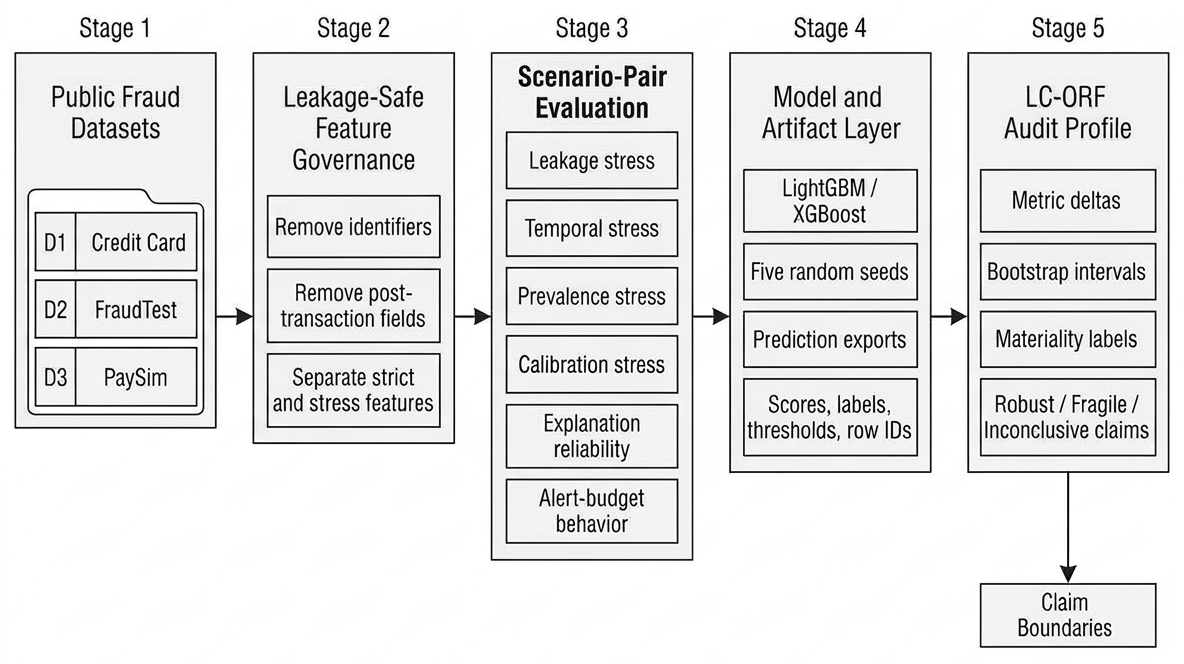
\includegraphics[width=0.95\textwidth]{figures/fig01_lcorf_framework_workflow.png}
\caption{LC-ORF operational robustness workflow. The same fraud-detection models are audited under controlled changes in leakage, temporal protocol, prevalence, calibration, explanation behavior, and alert-budget assumptions.}
\label{fig:workflow}
\end{figure*}

\subsection{Protocol Summary}
The protocol is written as a claim-audit procedure. Each run starts from a strict reference protocol, changes one assumption at a time, and records whether the resulting change is practically material. This keeps the audit interpretable: when a result moves, the paper can point to the assumption that moved it.

\begin{figure}[!htbp]
\centering
\fbox{%
\begin{minipage}{0.94\columnwidth}
\scriptsize
\textbf{Algorithm 1: LC-ORF scenario-pair audit protocol}

\vspace{1mm}
\textbf{Input:} datasets $\mathcal{D}$, models $\mathcal{M}$, seeds $\mathcal{S}$, audit axes $\mathcal{A}$, metrics $\mathcal{K}$, materiality thresholds $T_k$, bootstrap count $B$.

\textbf{Output:} audit profile with deltas, uncertainty summaries, materiality labels, alert-budget evidence, and claim boundaries.

\begin{enumerate}[leftmargin=*,topsep=1pt,itemsep=0pt]
\item Define strict scoring-time features and the safe reference protocol for each dataset.
\item For each audit axis, define a reference scenario $c_0$ and a one-assumption perturbation $c_1$.
\item Train or reuse each $(d,m,s,c)$ artifact and export labels, scores, thresholds, split, scenario, and row metadata.
\item Compute $\Delta_{a,d,m,s,k}=Q_k(c_1)-Q_k(c_0)$ for every metric with the correct metric direction.
\item Estimate uncertainty with paired or stratified bootstrap where applicable; use deterministic summaries for prevalence stress.
\item Assign robust, fragile, or inconclusive labels, then join all rows into the final LC-ORF profile.
\end{enumerate}
\end{minipage}}
\caption{LC-ORF audit protocol. The procedure treats the evaluation design as part of the scientific claim and records how conclusions change when one operational assumption is perturbed.}
\label{alg:lcorf_protocol}
\end{figure}

\subsection{Audit Units and Scenario Pairs}
Let $\mathcal{D}$ denote the datasets, $\mathcal{M}$ the model families, $\mathcal{S}$ the random seeds, $\mathcal{A}$ the audit axes, and $\mathcal{K}$ the metrics. An audit unit is indexed by $(d,m,s,a,c_0,c_1,k)$, where $d \in \mathcal{D}$, $m \in \mathcal{M}$, $s \in \mathcal{S}$, $a \in \mathcal{A}$, $c_0$ is a reference scenario, $c_1$ is a perturbed scenario, and $k \in \mathcal{K}$ is a metric. In this study, $\mathcal{D}$ contains D1\_creditcard, D2\_fraudTest, and D3\_PaySim; $\mathcal{M}$ contains LightGBM and XGBoost; and $\mathcal{S}=\{42,101,202,303,404\}$.

\begin{table}[!htbp]
\caption{LC-ORF Audit Axes and Claim Boundaries}
\label{tab:audit_axes}
\centering
\scriptsize
\setlength{\tabcolsep}{2pt}
\renewcommand{\arraystretch}{1.08}
\begin{tabularx}{\columnwidth}{|>{\raggedright\arraybackslash}p{0.19\columnwidth}|>{\raggedright\arraybackslash}p{0.34\columnwidth}|>{\raggedright\arraybackslash}X|}
\hline
\textbf{Axis} & \textbf{Changed assumption} & \textbf{Claim boundary}\\
\hline
Leakage & Unsafe preprocessing or ledger-state access & Shows sensitivity to leakage-prone evaluation; not a new classifier.\\
\hline
Temporal & Random stratified split versus chronological evaluation & Shows degradation under this benchmark protocol; not proof of all deployment drift.\\
\hline
Prevalence & Fraud-rate composition in the evaluation stream & Shows base-rate sensitivity; not prevalence-invariant modeling.\\
\hline
Calibration & Raw scores versus Platt or isotonic recalibration & Shows probability-quality behavior; not guaranteed cost reduction.\\
\hline
Explanation protocol & Random explanation protocol versus chronological protocol & Reports an explanation reliability proxy; not causal explanation validation.\\
\hline
Alert budget & Fixed alert capacity and score thresholds & Reports workload behavior under chosen budgets; not an optimized bank policy.\\
\hline
\end{tabularx}
\end{table}

Table~\ref{tab:scenario_pairs} makes the scenario-pair construction explicit. The reference scenario is the condition under which the original claim should be trusted; the perturbed scenario is the stress condition used to test whether that claim changes. This table is included because the scenario definition is part of the method, not a notebook detail.

\begin{table}[!htbp]
\caption{Scenario-Pair Definitions Used by LC-ORF}
\label{tab:scenario_pairs}
\centering
\scriptsize
\setlength{\tabcolsep}{2pt}
\renewcommand{\arraystretch}{1.08}
\begin{tabularx}{\columnwidth}{|>{\raggedright\arraybackslash}p{0.19\columnwidth}|>{\raggedright\arraybackslash}p{0.25\columnwidth}|>{\raggedright\arraybackslash}p{0.25\columnwidth}|>{\raggedright\arraybackslash}X|}
\hline
\textbf{Axis} & \textbf{Reference scenario} & \textbf{Perturbed scenario} & \textbf{Claim tested}\\
\hline
Leakage & Strict features and resampling inside training fold & SMOTE-before-split or D3 ledger-state stress & Whether reported skill is inflated by unavailable information.\\
\hline
Temporal & Random stratified safe split & Chronological safe split & Whether the conclusion holds under future-like evaluation.\\
\hline
Prevalence & Original evaluation stream & Resampled target fraud-rate streams & Whether operating metrics remain stable when base rate changes.\\
\hline
Calibration & Raw model scores & Platt sigmoid or isotonic recalibration & Whether probability-quality gains change operating conclusions.\\
\hline
Explanation & Random-split explanation protocol & Chronological explanation protocol & Whether explanation rankings remain reliable when prediction behavior shifts.\\
\hline
Alert budget & Validation-selected threshold view & Fixed review budgets per 10,000 transactions & Whether model scores translate into usable investigation workload.\\
\hline
\end{tabularx}
\end{table}

For each metric $k$, LC-ORF defines the scenario delta as
\begin{equation}
\Delta_{a,d,m,s,k}
= Q_k(d,m,s,c_1) - Q_k(d,m,s,c_0),
\label{eq:delta}
\end{equation}
where $Q_k$ is the metric functional computed from true labels, model scores, and the decision threshold. The sign convention is perturbed minus reference. A positive leakage delta therefore means that the unsafe protocol increased the measured metric relative to the strict protocol. A negative temporal delta means chronological evaluation reduced the metric relative to random stratified evaluation. For Brier score, ECE, and cost, lower values are better, so the sign must be interpreted according to metric direction.

Each scenario-pair row is therefore a bounded claim, not a free-standing model score. The final profile records the dataset, model, seed, reference scenario, perturbed scenario, metric, metric direction, bootstrap mode, evidence type, and materiality label. This record matters because two rows can have the same numerical delta but different evidential status: one may be paired at the row level, another may require stratified unpaired resampling, and a third may be a deterministic prevalence stress summary. LC-ORF keeps these differences visible so that the paper does not convert heterogeneous evidence into a single leaderboard.

\subsection{Uncertainty and Materiality}
For leakage, temporal, calibration, and explanation-protocol comparisons, LC-ORF uses $B=1000$ bootstrap replicates. When reference and perturbed predictions share row-level alignment, paired bootstrap resampling is used. Otherwise, LC-ORF uses stratified unpaired resampling to preserve label composition within each scenario. For bootstrap replicate $b$,
\begin{equation}
\Delta^{(b)}_{a,d,m,s,k}
= Q^{(b)}_k(d,m,s,c_1) - Q^{(b)}_k(d,m,s,c_0).
\end{equation}
The interval is the percentile interval
\begin{equation}
CI_{a,d,m,s,k}
= [P_{2.5}(\Delta^{(1:B)}), P_{97.5}(\Delta^{(1:B)})].
\end{equation}

LC-ORF assigns robust, fragile, or inconclusive labels using materiality thresholds $T_k$. In this study, $T_{AP}=0.020$, $T_{MCC}=0.050$, $T_{precision}=0.050$, $T_{recall}=0.050$, $T_{Brier}=0.005$, $T_{ECE}=0.020$, and $T_{cost}=\max(100,0.10|Q_{cost}(c_0)|)$. A comparison is robust when both interval endpoints lie inside the materiality band. It is fragile when the whole interval lies beyond the band in the same direction. All other cases are inconclusive.

\subsection{Prevalence, Alert-Budget, and Explanation Components}
The prevalence component evaluates fixed models and thresholds under altered fraud-rate composition in the evaluation stream. It reports the mean delta across target prevalence levels, the worst target prevalence, and the maximum absolute delta.

The alert-budget component ranks transactions by score and evaluates fixed investigation budgets. The reported quantities are alert precision, alert recall, false alerts, and estimated cost. This makes the profile operationally meaningful: a model score is connected to the number and quality of alerts a fraud team would review.

The explanation reliability gap is an artifact-level proxy. Let $\overline{J}^{(top-k)}_{d,m}$ be the mean top-$k$ Jaccard agreement between explanation feature rankings under compared protocols. LC-ORF defines
\begin{equation}
EII_{d,m}=1-\overline{J}^{(top-k)}_{d,m}.
\end{equation}
Using $k=5$ and $T_{AP}=0.020$, the AP fragility unit is
\begin{equation}
F^{AP}_{d,m}
= \frac{|\Delta^{AP}_{explanation,d,m}|}{T_{AP}}.
\end{equation}
The explanation reliability gap is
\begin{equation}
ERG_{d,m}=F^{AP}_{d,m}-EII_{d,m}.
\label{eq:erg}
\end{equation}
An $ERG$ above 1 indicates that predictive degradation exceeds explanation-rank instability by at least one AP materiality unit. This should not be interpreted as causal explanation validation.

\FloatBarrier
\section{Experimental Design}
\label{sec:design}
\subsection{Datasets and Governance}
The study uses three public fraud datasets. D1 is the European credit-card dataset distributed through Kaggle and associated with the ULB Machine Learning Group \cite{creditcard_kaggle}. D2 is the simulated merchant card transaction dataset distributed as \texttt{fraudTest.csv} \cite{fraudtest_kaggle}. D3 is PaySim, a mobile-money fraud simulation dataset \cite{lopezrojas2016paysim}.

Feature governance is applied before modeling. Identifier-like fields, personal names, transaction numbers, and fields not available at scoring time are excluded from the strict protocol. For D3, ledger-state balance fields whose availability depends on the scoring moment are excluded from strict features and used only as a leakage stress condition. This governance step is part of the method, because a fraud model cannot rely on variables that are unavailable when a decision is made.

The strict protocol follows three rules. First, variables that directly identify a customer, merchant, transaction, or synthetic account are not used as predictive features. Such variables can act as memorization keys, especially under random splitting. Second, variables created after the transaction outcome are excluded from strict evaluation, even when they are present in the public data file. This rule is most important for D3, where ledger-state balance fields can encode information that would not be available before a decision is made. Third, resampling is treated as a training-only operation. SMOTE-before-split is not used as a valid modeling protocol; it is included only as a leakage stress condition because it can let synthetic minority examples influence both training and test distributions.

The same governance logic is applied across datasets, but the available fields differ. D1 is already anonymized, so the main risk is evaluation design rather than named identifiers. Its \texttt{Time} field is an elapsed source-time variable rather than a full calendar timestamp; temporal conclusions on D1 are therefore treated as source-order robustness evidence, not as a bank deployment forecast. D2 contains richer transaction descriptors and temporal fields, so the chronological protocol is more directly future-like. D3 is synthetic and large, but its ledger-state variables make it useful for testing how strong a model can appear when state fields unavailable at decision time are allowed. Several D3 stress calculations use a timeline-preserving subset for computational feasibility, so D3 evidence is reported as synthetic large-stream stress evidence rather than real-world banking evidence. These differences are the reason LC-ORF reports dataset-specific evidence instead of collapsing the three datasets into one leaderboard.

\begin{table}[!t]
\caption{Dataset Summary of Evaluation Artifacts}
\label{tab:datasets}
\centering
\small
\renewcommand{\arraystretch}{1.10}
\begin{tabular}{|l|r|r|r|}
\hline
\textbf{Dataset} & \textbf{Rows} & \textbf{Fraud rows} & \textbf{Fraud rate}\\
\hline
D1\_creditcard & 284,807 & 492 & 0.173\%\\
\hline
D2\_fraudTest & 555,719 & 2,145 & 0.386\%\\
\hline
D3\_PaySim & 5,840,046 & 4,497 & 0.077\%\\
\hline
\end{tabular}
\end{table}

The counts in Table~\ref{tab:datasets} describe the cleaned evaluation artifacts used in this study after dataset-specific governance and validity checks. They should not be read as a claim that every public source file has the same raw row count.

\subsection{Models, Metrics, and Artifacts}
The framework is instantiated with LightGBM and XGBoost. These are strong tabular learners, but they are not the novelty of the paper. The five random seeds are 42, 101, 202, 303, and 404. The metrics are AP, MCC, precision, recall, Brier score, ECE, and cost per 10,000 transactions. Thresholded metrics use validation-selected cost-sensitive thresholds with false-negative cost set higher than false-positive cost in the experimental artifacts. The cost ratio is an experimental stress assumption, not a measured loss model from a bank or payment provider.

Each milestone exports prediction files with dataset, model, scenario, seed, split, row identifier, true label, score, and threshold columns. The final LC-ORF profile is built from these exported predictions rather than from untracked notebook state. This improves traceability and allows bootstrap comparisons across saved prediction artifacts. It also prevents a common reproducibility weakness in notebook-based fraud studies: a table can be regenerated from stored labels and scores without rerunning the entire training pipeline.

\subsection{Reproducibility and Artifact Workflow}
LC-ORF is implemented as an artifact-first workflow. Each experimental milestone writes its own prediction exports, metric summaries, figures, logs, and checkpoints before the final profile is assembled. The final analysis does not recompute hidden intermediate state from memory. It reads the saved artifacts and checks that the required columns are present before computing deltas, bootstrap intervals, or prevalence profiles.

This design has two practical benefits. First, it makes the audit recoverable when a cloud notebook disconnects or a GPU session expires; completed prediction exports and bootstrap checkpoints can be reused. Second, it gives the manuscript a clear chain from raw evaluation protocol to final claim. A reported delta can be traced back to the dataset, model, seed, scenario pair, metric, and prediction file used to compute it.

The artifact workflow also limits overclaiming. Rows that come from complete prediction exports are marked as complete evidence. Rows that use available explanation artifacts but do not constitute causal explanation validation are marked as proxy evidence. This distinction is preserved in the final profile so that the paper does not present every row with the same evidential strength.

\section{Results}
\label{sec:results}
\subsection{Final Audit Profile}
Figure~\ref{fig:audit_profile} shows the final audit profile. The profile contains 252 rows: 84 calibration rows, 42 leakage rows, 42 temporal rows, 42 explanation-protocol rows, 36 prevalence rows, and 6 explanation-reliability-gap rows. Of these, 246 rows have complete evidence, while 6 explanation-gap rows are marked as complete proxy evidence from existing artifacts.

The profile is meant to be read as a claim audit rather than as a ranking table. A red or blue cell is not, by itself, a success or failure. It shows that a measured quantity changed when one operational assumption was perturbed. The relevant question is then whether the change is material for the claim being made. For this reason, LC-ORF keeps metric direction, materiality thresholds, and evidence type attached to each profile row.

\begin{figure*}[!t]
\centering
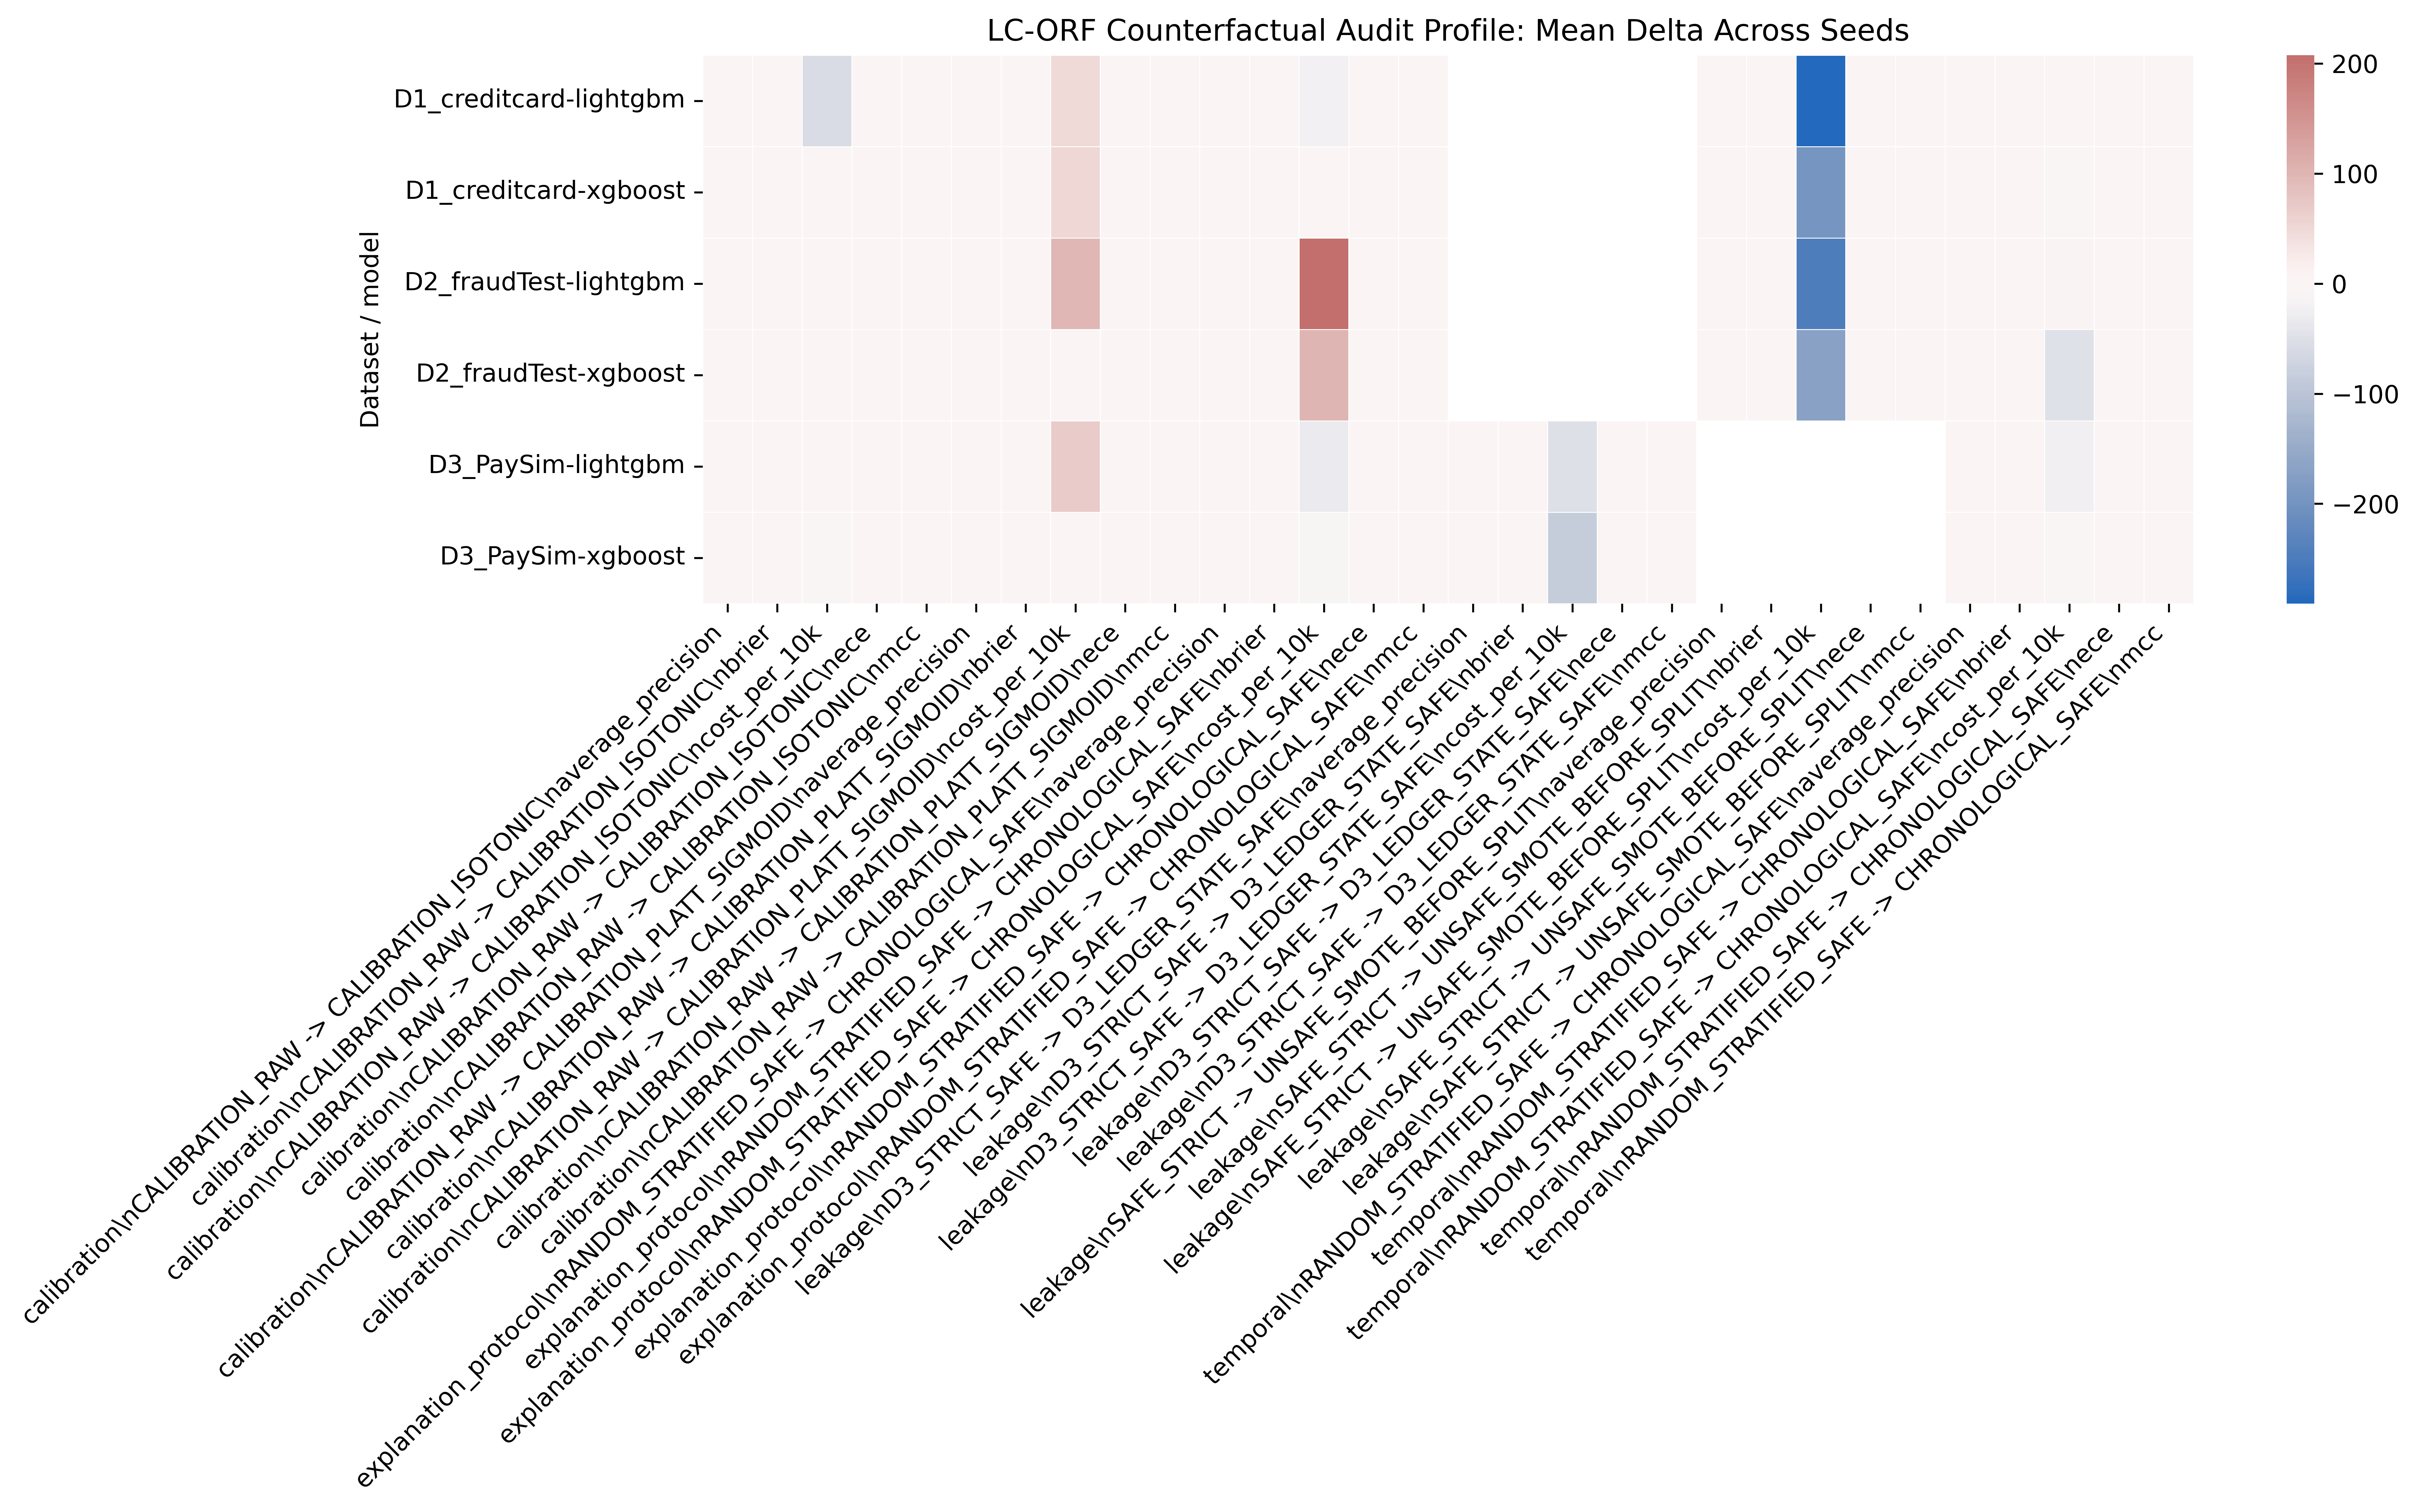
\includegraphics[width=0.95\textwidth]{figures/fig02_lcorf_final_audit_profile_heatmap.png}
\caption{Final LC-ORF audit profile heatmap. The profile reports leakage, temporal, prevalence, calibration, explanation-protocol, and explanation-reliability evidence across datasets and models.}
\label{fig:audit_profile}
\end{figure*}

\begin{table}[!t]
\caption{Final Audit-Profile Coverage}
\label{tab:profile_summary}
\centering
\small
\renewcommand{\arraystretch}{1.10}
\begin{tabular}{|l|r|r|r|}
\hline
\textbf{Axis} & \textbf{Rows} & \textbf{Datasets} & \textbf{Models}\\
\hline
Calibration & 84 & 3 & 2\\
\hline
Explanation protocol & 42 & 3 & 2\\
\hline
Leakage & 42 & 3 & 2\\
\hline
Temporal & 42 & 3 & 2\\
\hline
Prevalence & 36 & 3 & 2\\
\hline
Explanation reliability gap & 6 & 3 & 2\\
\hline
\end{tabular}
\end{table}

\subsection{Leakage Inflation}
The leakage audit shows the largest effects under unsafe SMOTE-before-split evaluation. D2 XGBoost produced an MCC inflation of 0.472, D2 LightGBM produced 0.361, and D1 XGBoost produced 0.357. AP also increased under unsafe leakage-prone protocols, including 0.142 for D1 XGBoost and 0.140 for D1 LightGBM.

The leakage result is strongest on D1 and D2 because the unsafe stress directly changes the evaluation pipeline through resampling before the split. This is not a subtle effect. A model can appear much stronger when synthetic minority examples are created before train-test separation, because information from the eventual test distribution can influence the training distribution. LC-ORF does not treat that condition as a valid model improvement. It uses it as a stress test to quantify how much a careless protocol can inflate the reported conclusion.

For D3, the leakage stress is different. The main issue is not SMOTE-before-split but the availability of ledger-state variables that are not appropriate for strict scoring-time evaluation. The D3 results therefore answer a narrower question: how much the conclusion changes when post-transaction state is allowed. This distinction is important because leakage is not a single failure mode. It can enter through resampling, feature timing, row identity, or state variables.

\begin{figure}[!t]
\centering
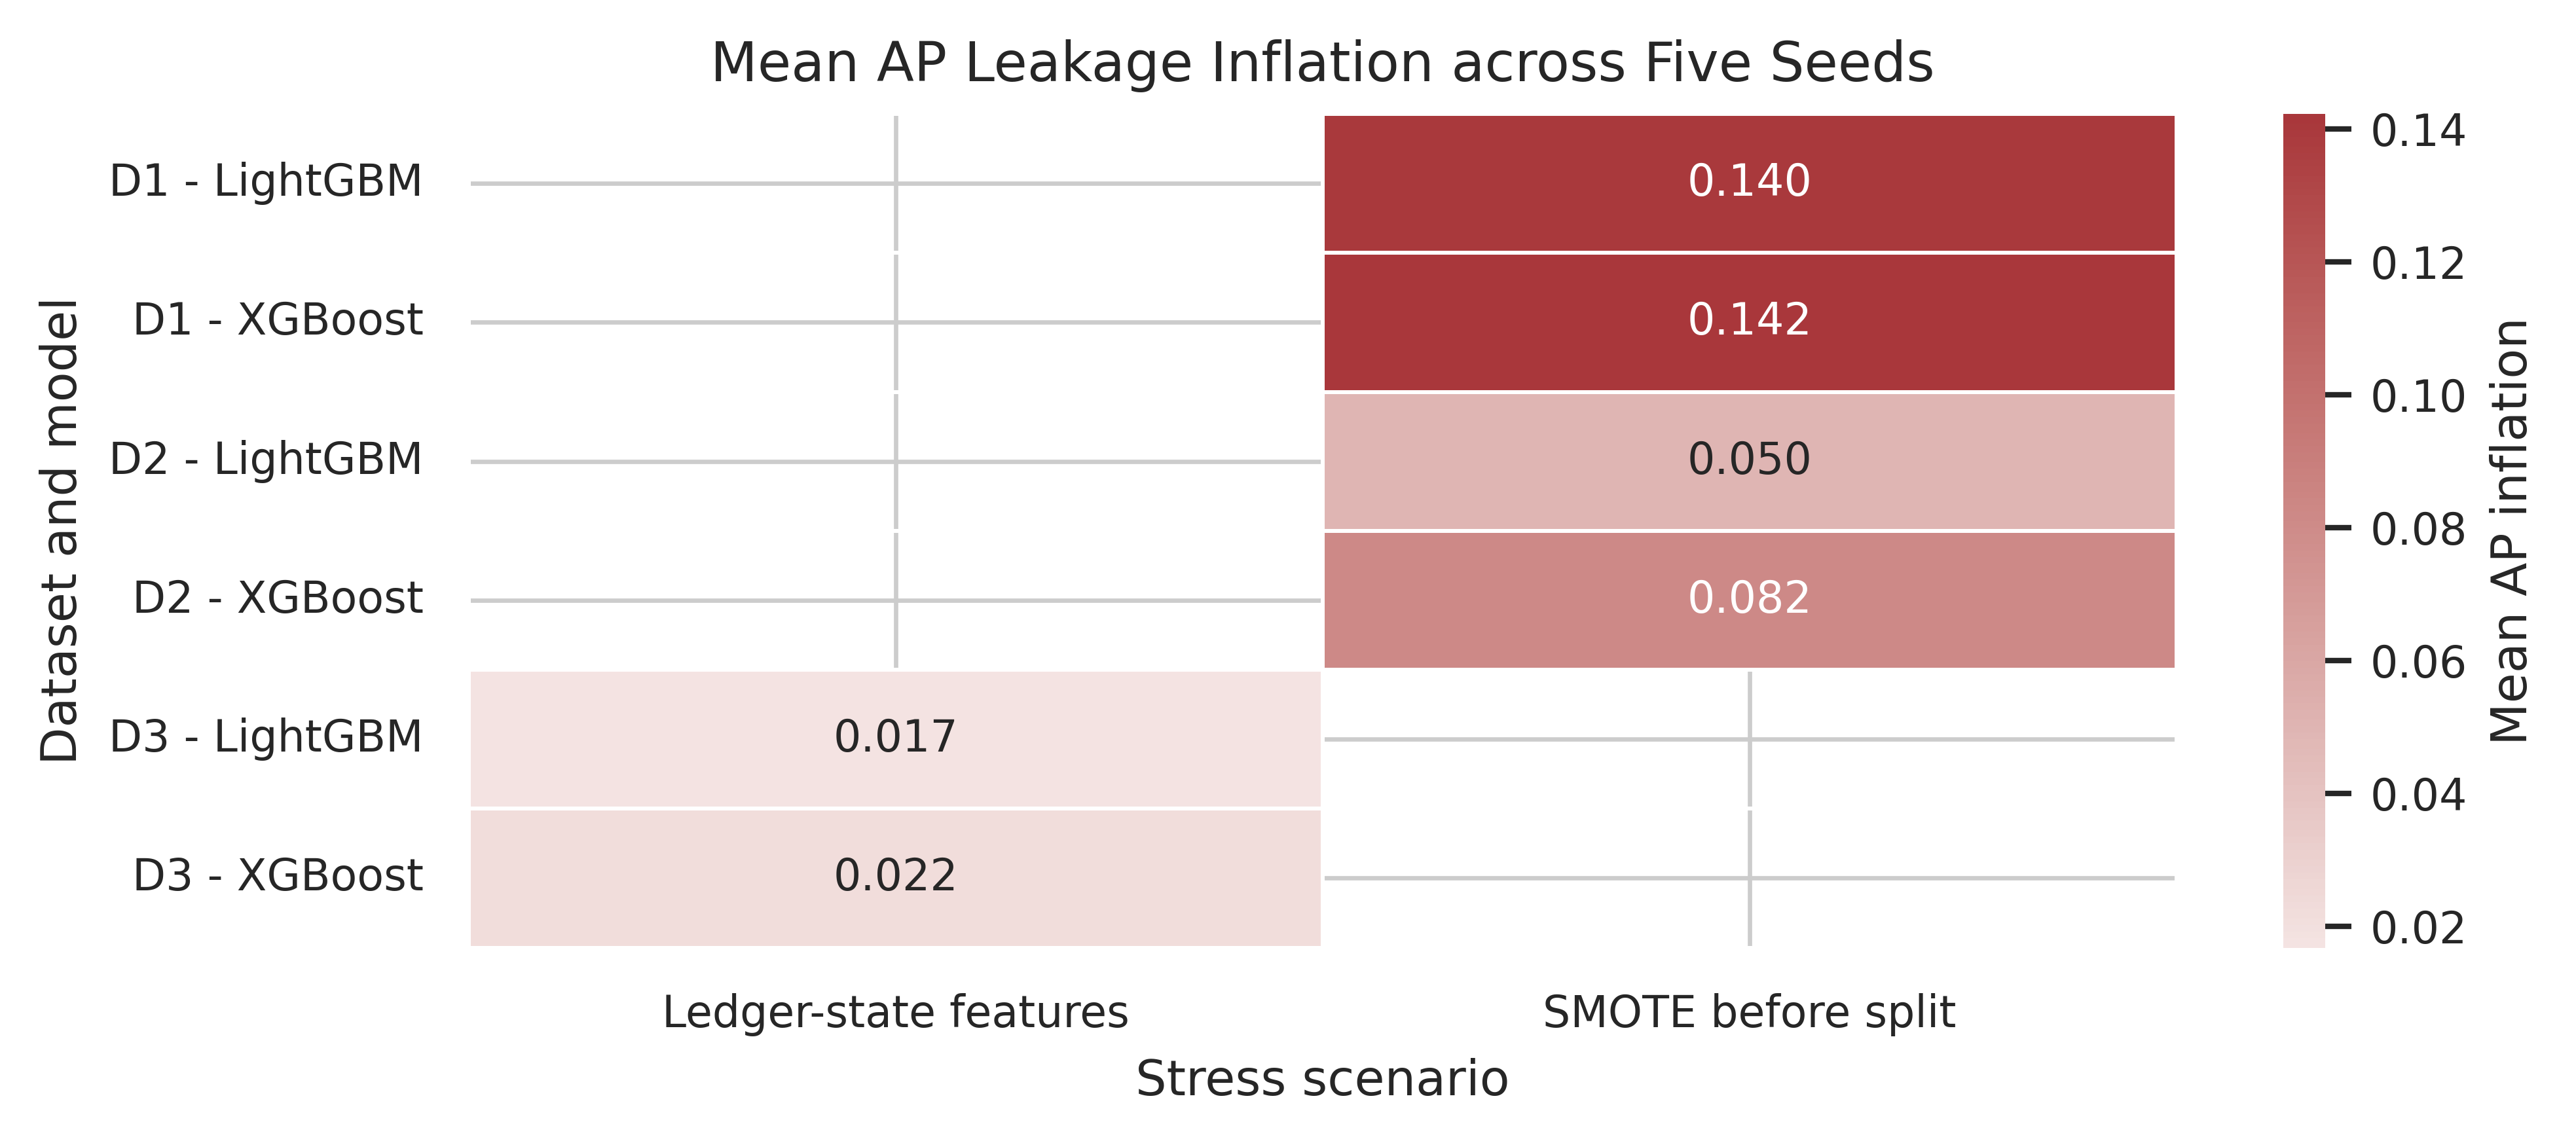
\includegraphics[width=\columnwidth]{figures/fig03_multiseed_ap_leakage_inflation_heatmap.png}
\caption{Multi-seed AP leakage inflation. Unsafe protocols can make the same model appear substantially stronger than it is under strict evaluation.}
\label{fig:leakage}
\end{figure}

\begin{table}[!t]
\caption{Representative Bootstrap-Backed Findings}
\label{tab:key_bootstrap}
\centering
\small
\renewcommand{\arraystretch}{1.08}
\begin{tabular}{|l|l|l|r|}
\hline
\textbf{Axis} & \textbf{Dataset/model} & \textbf{Metric} & \textbf{Mean delta}\\
\hline
Leakage & D2 XGBoost & MCC & 0.472\\
\hline
Leakage & D2 LightGBM & MCC & 0.361\\
\hline
Leakage & D1 XGBoost & MCC & 0.357\\
\hline
Leakage & D1 XGBoost & AP & 0.142\\
\hline
Leakage & D1 LightGBM & AP & 0.140\\
\hline
Temporal & D2 XGBoost & AP & -0.277\\
\hline
Temporal & D2 LightGBM & AP & -0.245\\
\hline
Temporal & D2 LightGBM & MCC & -0.242\\
\hline
Temporal & D2 XGBoost & MCC & -0.208\\
\hline
\end{tabular}
\end{table}

This is the clearest reason the manuscript should not be presented as another model comparison. A high score under an unsafe protocol can be partly a property of the pipeline. LC-ORF makes that inflation measurable.

\subsection{Temporal Degradation}
D2 shows the strongest temporal degradation. Figure~\ref{fig:d2_drift} connects feature drift and chronological performance drop. The D2 fraud rate also falls across chronological splits: the train split has a fraud rate of 0.00468, the validation split has 0.00361, and the chronological test split has 0.00166.

This result is operationally important because a random stratified split can hide the harder question faced by a deployed detector. In a live setting, the model is normally trained on earlier behavior and evaluated on later behavior. D2 exposes that difference: the chronological test period has a lower fraud rate and a changed feature distribution, and the resulting AP and MCC are lower than under random stratification. The effect is therefore not only a metric artifact; it is tied to a different evaluation question.

\begin{figure*}[!t]
\centering
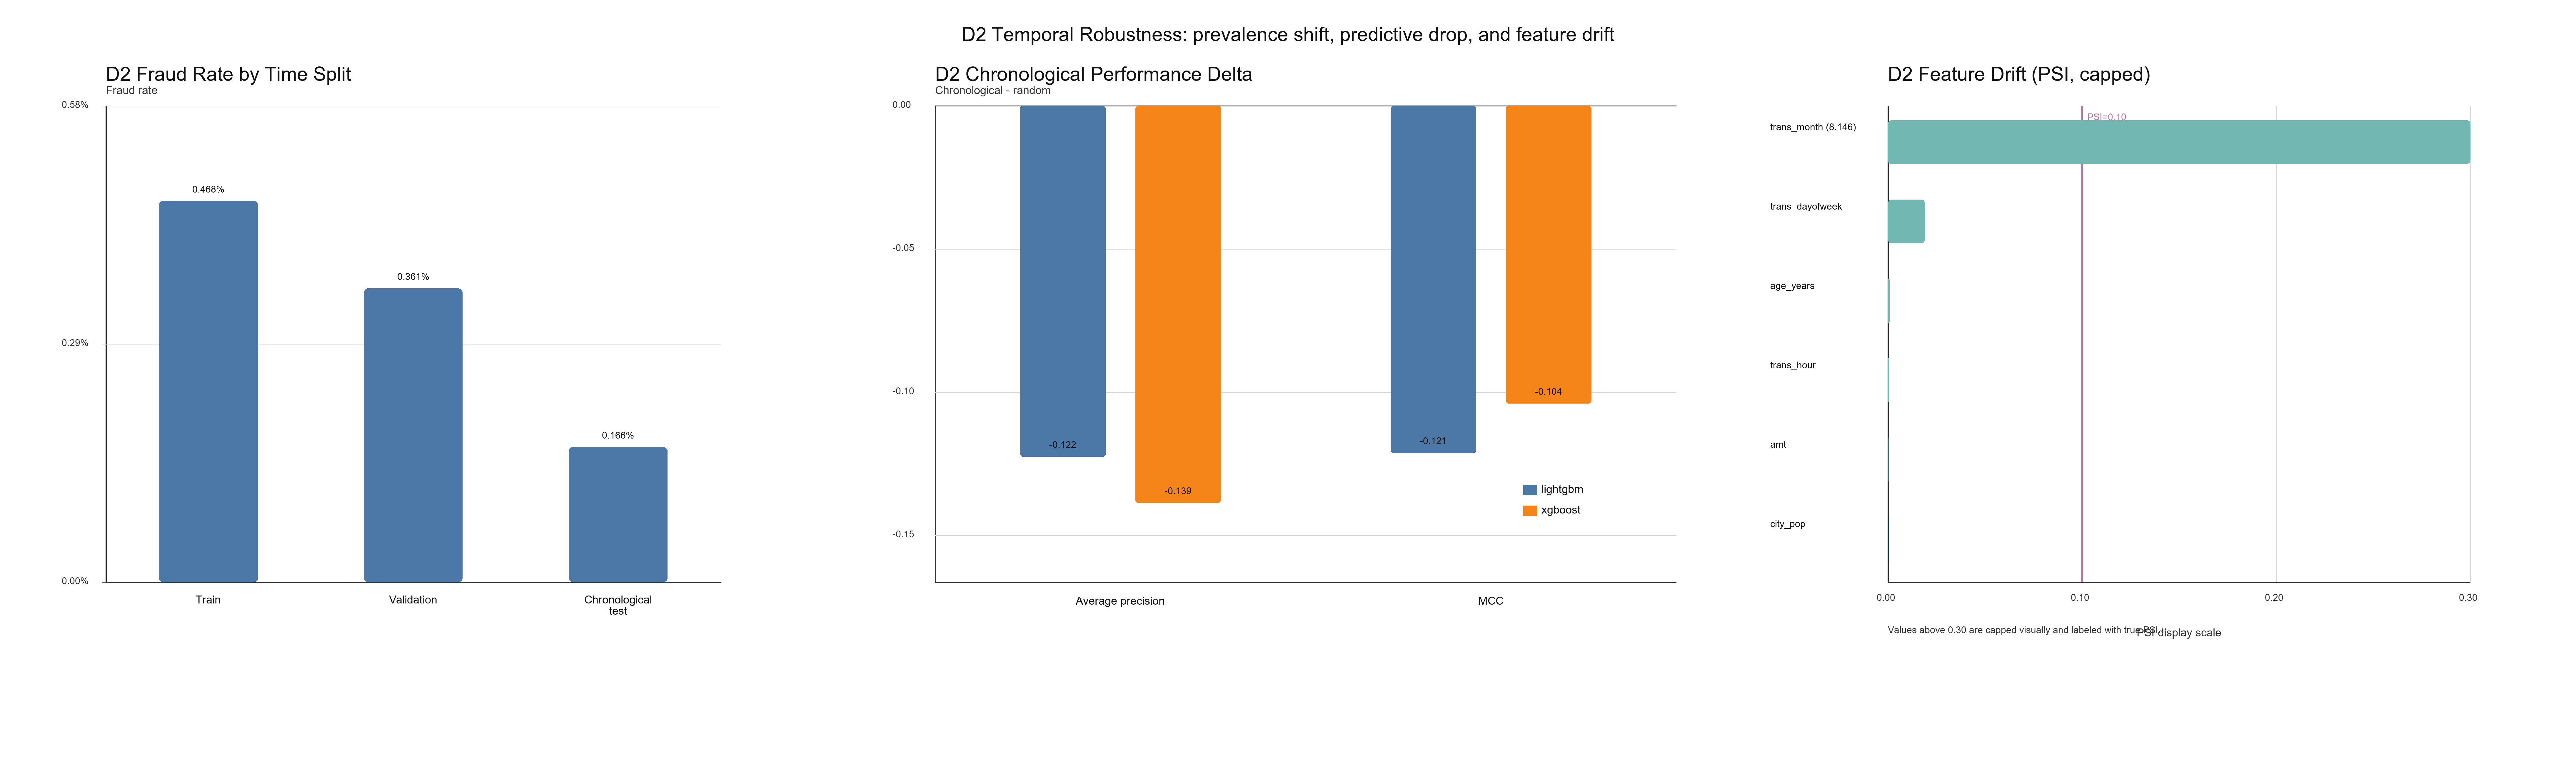
\includegraphics[width=0.85\textwidth]{figures/fig04_d2_drift_vs_temporal_drop.png}
\caption{D2 temporal drift and performance degradation. Chronological evaluation exposes a harder test condition than random stratified evaluation.}
\label{fig:d2_drift}
\end{figure*}

\begin{table}[!t]
\caption{D2 Chronological Prevalence by Split}
\label{tab:d2_prevalence}
\centering
\small
\renewcommand{\arraystretch}{1.10}
\begin{tabular}{|l|r|r|r|}
\hline
\textbf{Split} & \textbf{Rows} & \textbf{Fraud rows} & \textbf{Fraud rate}\\
\hline
Train & 333,431 & 1,560 & 0.00468\\
\hline
Validation & 111,144 & 401 & 0.00361\\
\hline
Chronological test & 111,144 & 184 & 0.00166\\
\hline
\end{tabular}
\end{table}

The temporal result should be stated carefully. It does not prove that every deployment will degrade by the same amount. It shows that, in D2, a future-like chronological protocol is materially harder than a random stratified protocol.

\subsection{Prevalence Sensitivity}
The prevalence profile shows that changing the fraud rate in the evaluation stream can materially alter the operating interpretation. The final prevalence component contains 36 rows; 29 are labeled fragile and 7 robust. Precision, MCC, and cost are especially sensitive because they depend strongly on the class base rate.

\begin{figure}[!t]
\centering
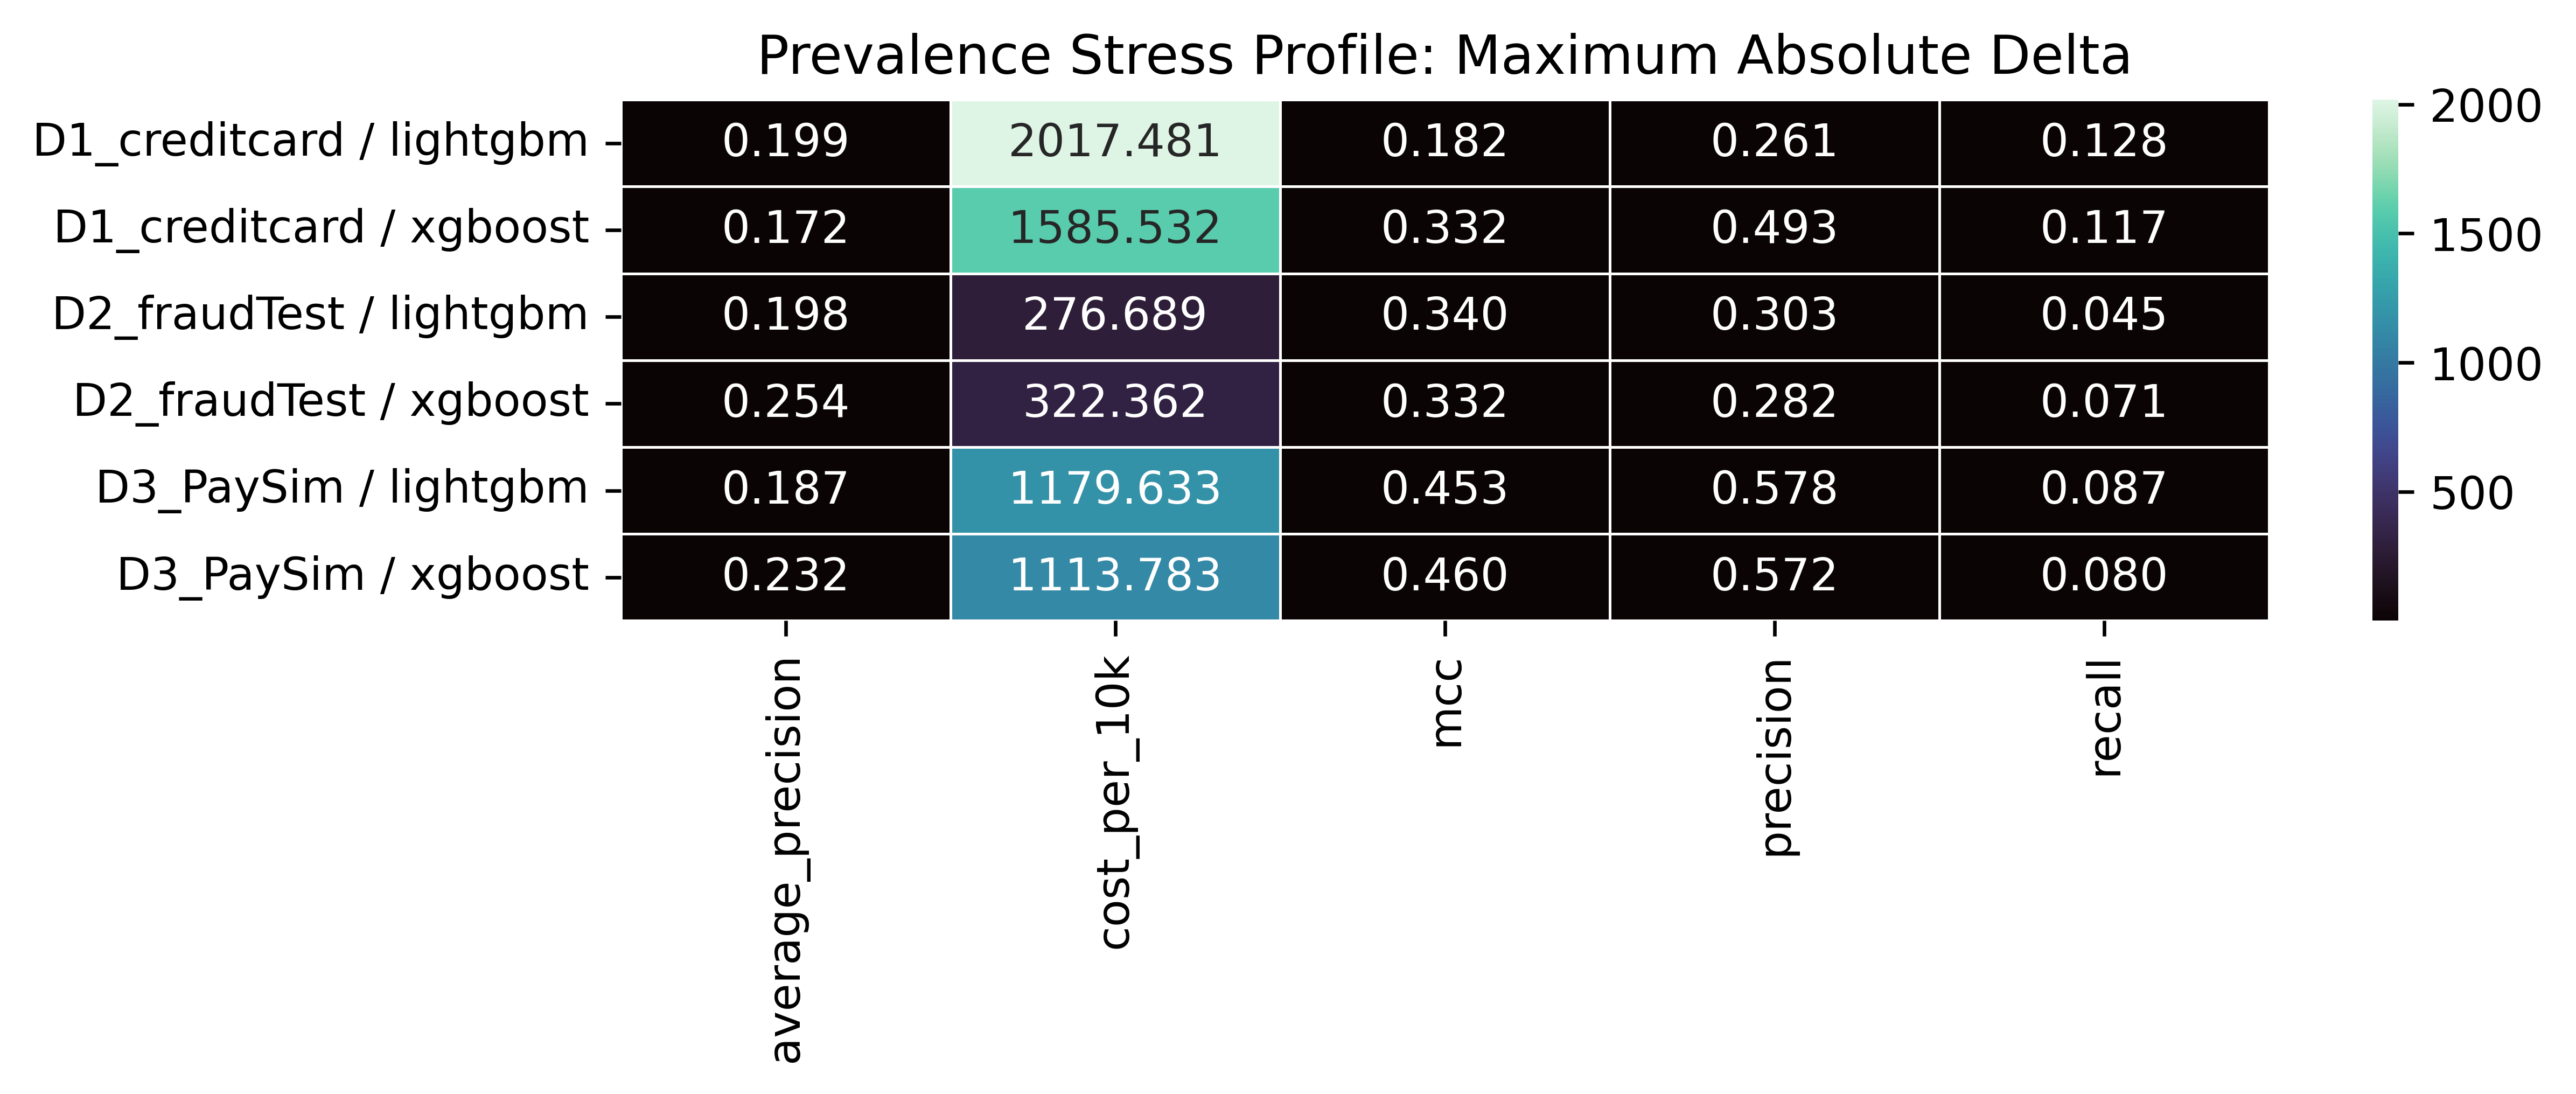
\includegraphics[width=\columnwidth]{figures/fig05_prevalence_profile_heatmap.png}
\caption{Prevalence profile heatmap. Fixed models and thresholds can produce materially different operating metrics under changed fraud-rate composition.}
\label{fig:prevalence}
\end{figure}

This result does not mean the classifier changes when prevalence changes. The model and threshold are fixed. The result means that downstream metrics such as precision and cost are functions of the stream composition. For fraud operations, that is still important because analyst workload and alert trust are driven by these operating metrics.

The practical consequence is that a fraud paper should not report one precision value as if it were independent of deployment prevalence. A screening system deployed in a stream with fewer fraudulent transactions can produce many more false alerts at the same threshold. Conversely, a higher-prevalence stream can make precision look better without any change in the model. LC-ORF makes this dependency visible by holding the model fixed and changing the evaluation stream.

\subsection{Calibration and Alert Budgets}
Calibration results are mixed in the correct way. Isotonic recalibration gives the best Brier and ECE behavior in the saved calibration artifacts across the dataset-model pairs considered here, but cost and thresholded metrics do not improve uniformly. This distinction matters because a calibrated score is not automatically an optimized fraud-investigation policy.

Table~\ref{tab:alert_budget} summarizes alert behavior under fixed budgets. This view is closer to fraud operations than a single aggregate AP value because a fraud team usually reviews a fixed number or fraction of transactions. The full-resolution alert-budget panel is retained in the supplementary artifact package rather than placed in the main paper, where it would be too dense at column scale.

The alert-budget result also explains why calibration is not enough on its own. A recalibrated model can produce probabilities that better match observed frequencies while still producing similar or worse behavior at a fixed investigation budget. Fraud teams usually face a capacity constraint: only a limited number of alerts can be reviewed. For that reason, LC-ORF reports alert precision, recall, false alerts, and cost summaries rather than relying only on score calibration metrics.

\begin{table}[!t]
\caption{Compact Alert-Budget Summary by Axis}
\label{tab:alert_budget}
\centering
\scriptsize
\setlength{\tabcolsep}{2pt}
\renewcommand{\arraystretch}{1.08}
\begin{tabular}{|l|r|r|r|r|}
\hline
\textbf{Axis} & \textbf{Groups} & \textbf{Mean precision} & \textbf{Mean recall} & \textbf{Mean false alerts}\\
\hline
Calibration & 6 & 0.113 & 0.943 & 4996.1\\
\hline
Explanation & 6 & 0.088 & 0.949 & 5042.3\\
\hline
Leakage & 6 & 0.635 & 0.582 & 1094.2\\
\hline
Prevalence & 6 & 0.113 & 0.948 & 4995.6\\
\hline
Temporal & 6 & 0.088 & 0.943 & 5043.3\\
\hline
\end{tabular}
\end{table}

\subsection{Explanation Reliability Gap}
The explanation analysis gives a useful caution. On D2, top-5 explanation rankings are stable under the available explanation artifacts, but predictive behavior shifts strongly under protocol changes. This produces a large explanation reliability gap: 10.841 for LightGBM and 11.659 for XGBoost. D3 has much smaller gaps, while D1 shows explanation-rank instability for LightGBM and a predictive-shift gap for XGBoost.

\begin{figure}[!htbp]
\centering
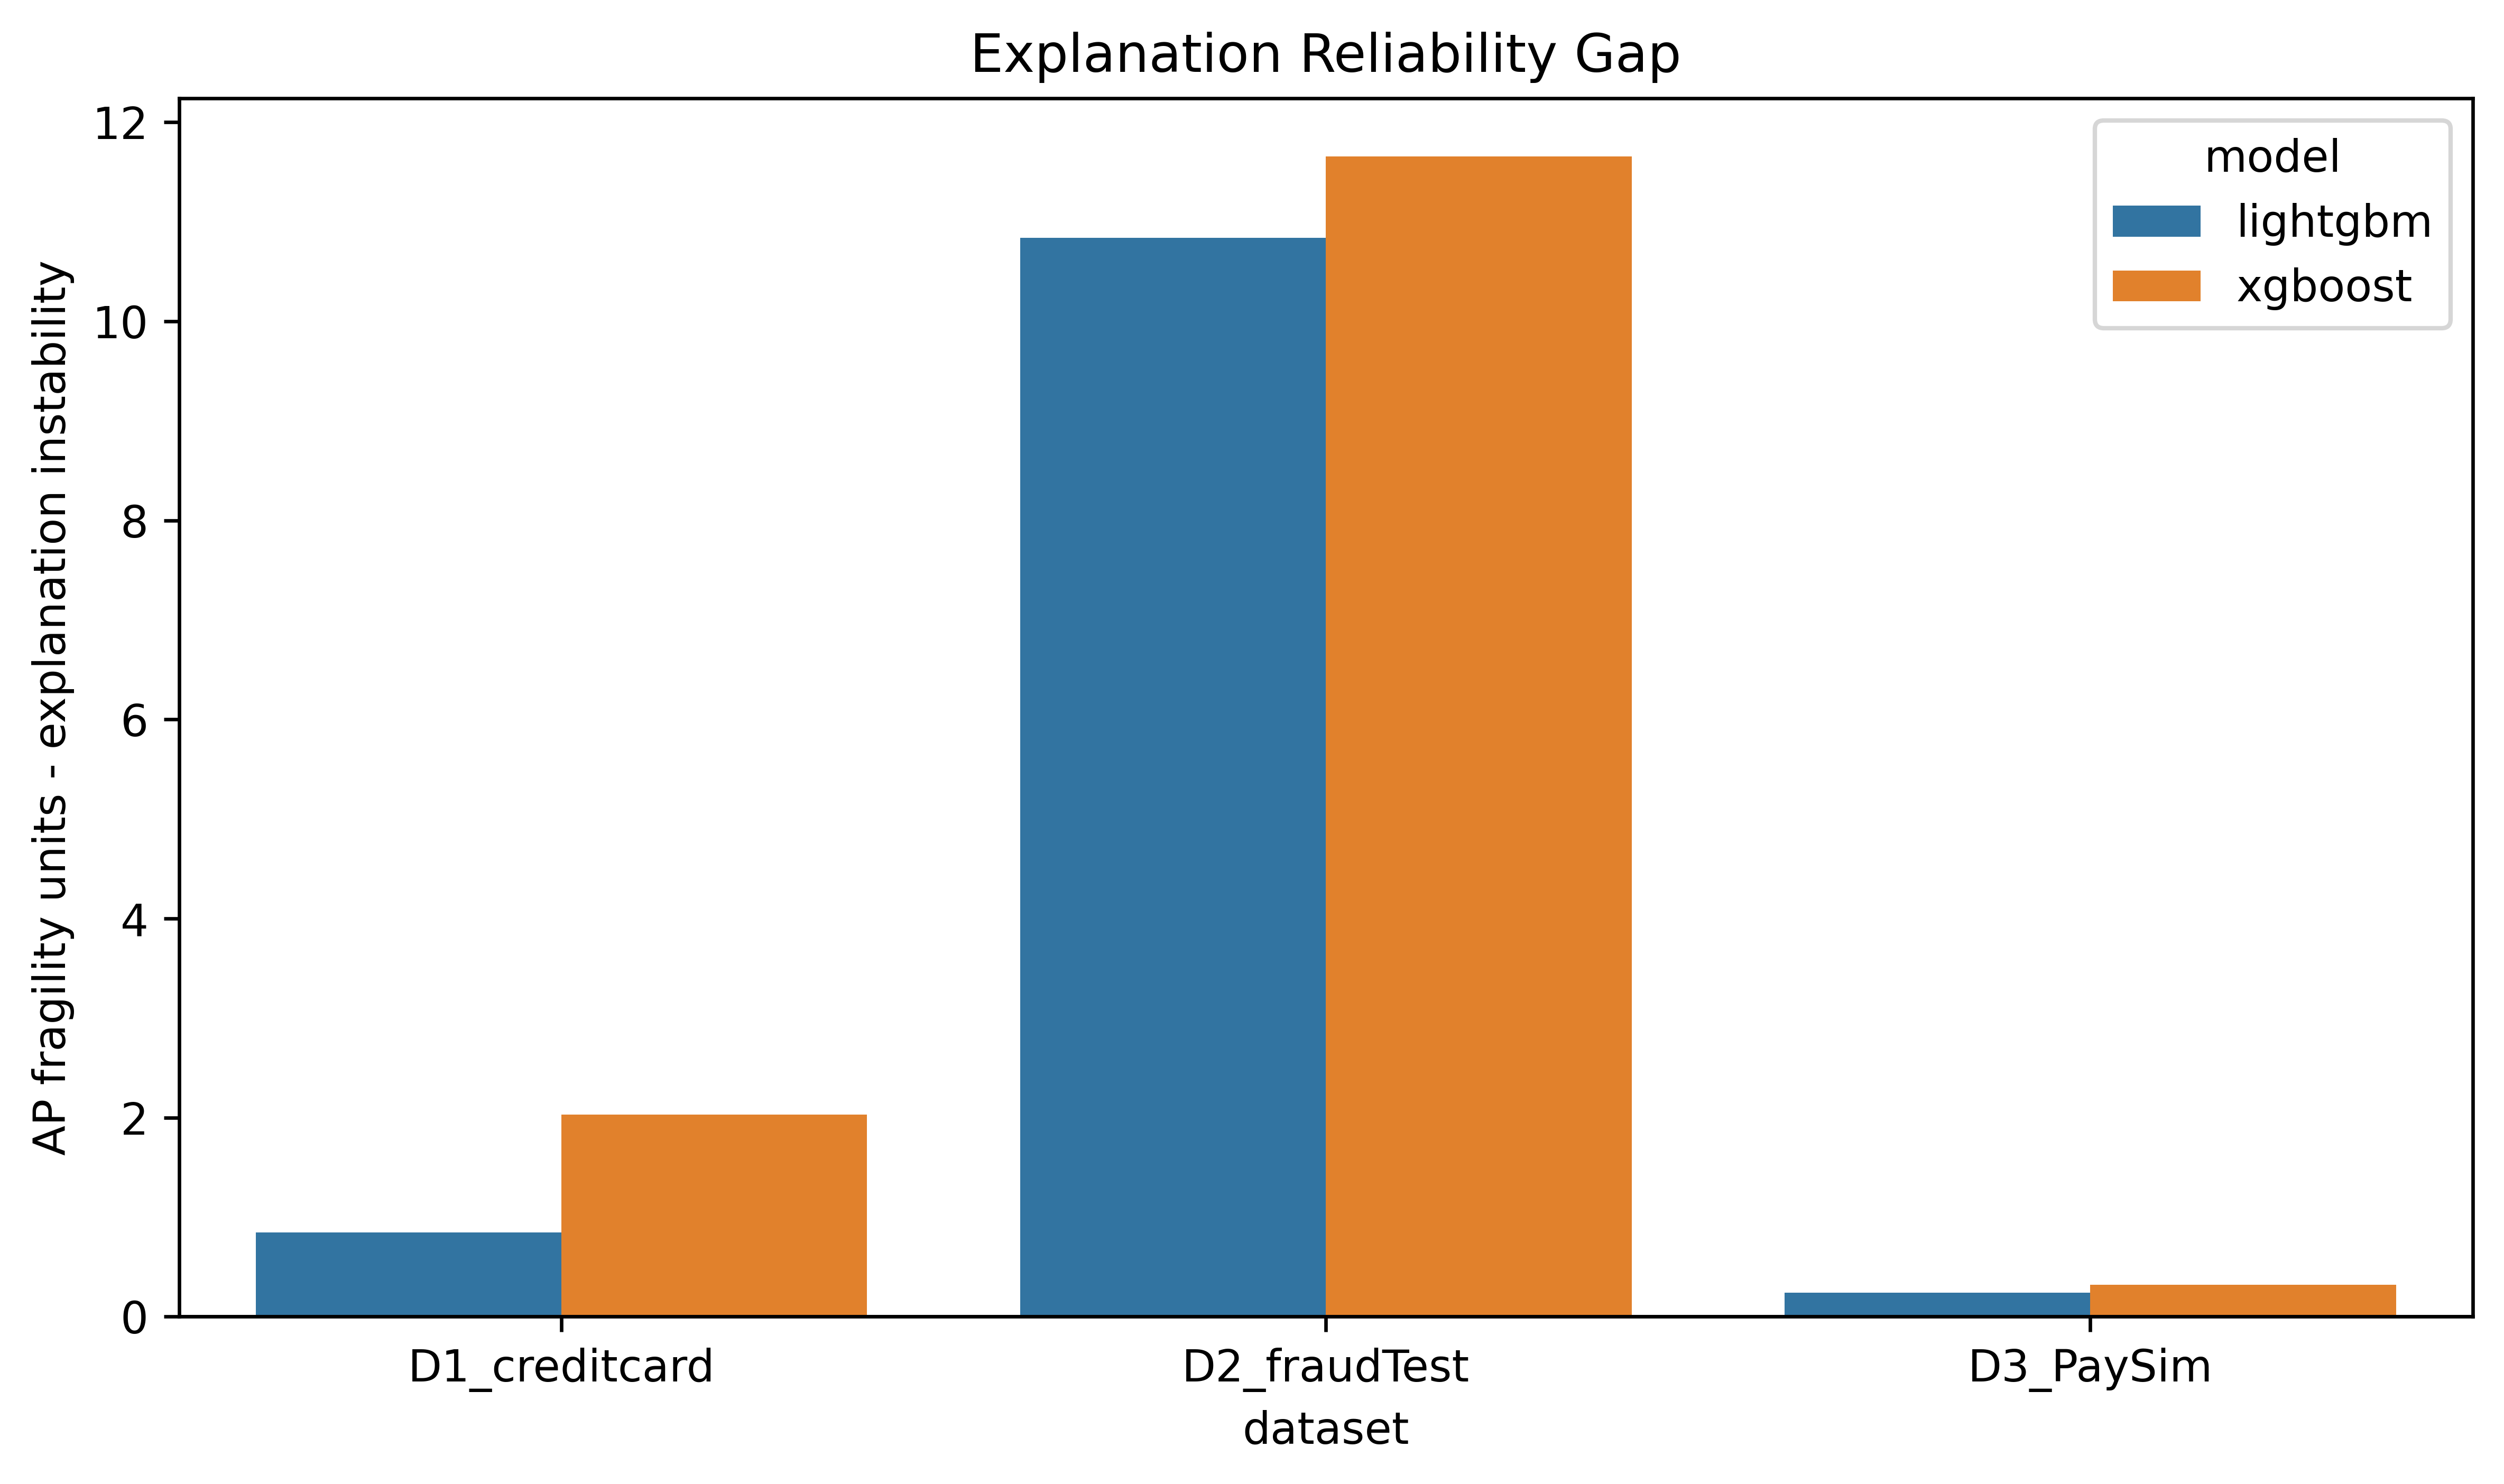
\includegraphics[width=0.80\columnwidth]{figures/fig07_explanation_reliability_gap.png}
\caption{Explanation reliability gap. The measure is an artifact-level proxy and should not be read as causal explanation validation.}
\label{fig:erg}
\end{figure}

\begin{table}[!t]
\caption{Explanation Reliability Gap}
\label{tab:erg}
\centering
\small
\renewcommand{\arraystretch}{1.10}
\begin{tabular}{|l|l|r|r|}
\hline
\textbf{Dataset} & \textbf{Model} & \textbf{EII} & \textbf{ERG}\\
\hline
D1 & LightGBM & 0.524 & 0.844\\
\hline
D1 & XGBoost & 0.248 & 2.032\\
\hline
D2 & LightGBM & 0.000 & 10.841\\
\hline
D2 & XGBoost & 0.000 & 11.659\\
\hline
D3 & LightGBM & 0.000 & 0.239\\
\hline
D3 & XGBoost & 0.000 & 0.319\\
\hline
\end{tabular}
\end{table}

The safe interpretation is narrow but important. Explanation rankings can appear stable while predictive behavior changes. Therefore explanation artifacts should be reported together with protocol-shift evidence, not as isolated interpretability claims.

This does not mean that SHAP-style or feature-rank explanations are useless. It means that explanation stability and predictive stability are different claims. A model may keep similar top-ranked features while its AP drops under chronological evaluation. In that case, the explanation artifact has not warned the reader that the predictive conclusion is fragile. LC-ORF separates those two issues so that explanation evidence is not used as a substitute for robustness evidence.

\FloatBarrier
\section{Framework Reuse and Extension}
\label{sec:reuse}
LC-ORF is intended to be reused, not only reproduced on the three datasets in this paper. A new fraud dataset can be added if four pieces are defined before modeling: the strict scoring-time feature set, the available split protocols, the leakage or stress condition to audit, and the exported prediction schema. These choices must be made before looking at the final performance deltas; otherwise, the audit can become another form of post-hoc model selection.

\begin{table}[!htbp]
\caption{Applying LC-ORF to a New Fraud Dataset}
\label{tab:reuse}
\centering
\scriptsize
\setlength{\tabcolsep}{2pt}
\renewcommand{\arraystretch}{1.10}
\begin{tabularx}{\columnwidth}{|>{\raggedright\arraybackslash}p{0.18\columnwidth}|>{\raggedright\arraybackslash}p{0.31\columnwidth}|>{\raggedright\arraybackslash}p{0.26\columnwidth}|>{\raggedright\arraybackslash}X|}
\hline
\textbf{Step} & \textbf{Decision required} & \textbf{Minimum artifact} & \textbf{Audit value}\\
\hline
Feature governance & Identify fields available at scoring time and remove identifiers or post-outcome variables. & Strict feature list and excluded-field list. & Prevents leakage from being hidden inside preprocessing.\\
\hline
Scenario design & Define $c_0$ and $c_1$ for each applicable audit axis. & Scenario registry with reference and perturbed protocols. & Makes each claim-changing assumption explicit.\\
\hline
Prediction export & Save labels, scores, thresholds, row identifiers, split, model, seed, and scenario. & Prediction CSV or equivalent table. & Allows the final profile to be rebuilt without notebook state.\\
\hline
Uncertainty policy & Select paired, stratified unpaired, or deterministic summary according to row alignment. & Bootstrap or stress-summary metadata. & Keeps confidence statements tied to the available evidence.\\
\hline
Claim reporting & Attach robust, fragile, or inconclusive labels to metric deltas. & Final LC-ORF profile. & Separates supported claims from fragile or proxy evidence.\\
\hline
\end{tabularx}
\end{table}

The framework can also be extended along two practical directions. First, the model layer can be replaced with any method that produces calibrated or uncalibrated scores: graph models, sequence models, online learners, or transformer-based tabular models can all be audited if they export the same prediction fields. LC-ORF does not require LightGBM or XGBoost. Those models are used here because they are strong tabular baselines and make the framework easier to inspect.

Second, the operational layer can be made institution-specific. A bank or payment platform could replace the illustrative cost assumptions with its own false-negative loss, false-positive review cost, review capacity, customer-friction penalty, and escalation rules. The profile would then answer a narrower and more useful question: not whether a model is generally strong, but whether its conclusion remains credible under that institution's operating constraints.

The reusable part of LC-ORF is therefore the discipline of the audit: define the reference claim, perturb one assumption at a time, export predictions, compute material deltas, and report the boundary of the claim. The individual thresholds and cost assumptions can change across deployments, but the profile should always preserve the link between a reported conclusion and the evaluation assumptions behind it.

\FloatBarrier
\section{Discussion}
\label{sec:discussion}
The results support the framework claim. LC-ORF reveals risks that a single performance table would hide. Leakage stress shows that unsafe preprocessing can inflate measured performance. Temporal stress shows that D2 is materially harder under chronological evaluation. Prevalence stress shows that operating metrics depend on fraud-rate composition. Calibration stress separates probability quality from thresholded cost. Explanation analysis shows that stable feature rankings do not necessarily imply stable predictive behavior.

\subsection{Reading the Profile by Dataset}
D1 is useful mainly as a leakage and rare-event evaluation case. Because D1 is anonymized and its time variable is an elapsed source-time field, the strongest D1 claim is not that the paper has reproduced a real future production stream. The stronger claim is narrower: even on a widely used anonymized benchmark, evaluation choices such as leakage-prone resampling can materially alter the reported conclusion. This is an important boundary because many fraud papers use D1 as a general benchmark without separating model performance from protocol quality.

D2 gives the clearest temporal lesson in this study. Its transaction descriptors and time structure allow a more direct random-versus-chronological comparison, and the chronological protocol materially reduces AP for both LightGBM and XGBoost. The D2 result is therefore the strongest evidence that a random stratified split can overstate operational usefulness. The claim is still bounded: it is evidence from this public transaction stream, not a universal drift magnitude for all institutions.

D3 has a different role. It is synthetic and much larger, so it is not treated as direct deployment evidence. Its value is methodological: the dataset contains ledger-state variables that make the leakage-governance question concrete. Under LC-ORF, D3 helps test whether a framework can separate strict scoring-time features from stress features whose availability would be questionable in a real decision setting. For computational feasibility, some D3 stress analyses use timeline-preserving subsets; this is why D3 conclusions are reported as synthetic stress evidence rather than bank-ready validation.

The prevalence findings should also be read operationally. A prevalence stress result does not mean that the trained model changed. It means the operating stream changed. Precision, false alerts, MCC, and cost can move because the same fixed threshold is applied to a stream with a different base rate. This is not a weakness of LC-ORF; it is the point of the prevalence axis. A fraud operation pays attention to the stream it receives, not only to the fitted score function.

\subsection{Operational Claim Audit}
Table~\ref{tab:claim_audit} summarizes the claim discipline enforced by LC-ORF. The table is deliberately conservative. It separates what the manuscript can claim from what would require institutional data, analyst studies, or deployment logs. This distinction is central to the novelty of the paper: the framework does not add metrics for their own sake; it ties each conclusion to the evidence needed to support it.

\begin{table*}[!t]
\caption{Operational Claim Audit Used by LC-ORF}
\label{tab:claim_audit}
\centering
\scriptsize
\setlength{\tabcolsep}{3pt}
\renewcommand{\arraystretch}{1.15}
\begin{tabularx}{\textwidth}{|>{\raggedright\arraybackslash}p{0.23\textwidth}|>{\raggedright\arraybackslash}p{0.37\textwidth}|>{\raggedright\arraybackslash}X|}
\hline
\textbf{Claim type} & \textbf{Minimum LC-ORF evidence} & \textbf{Boundary on the conclusion}\\
\hline
Scoring-time feature validity & Strict feature-governance table, excluded-field list, and scenario label showing that identifier-like and post-outcome fields are not used in the strict protocol. & Supports the claim that the reported strict result avoids known feature-availability leakage; it does not prove compliance with a specific bank's internal feature policy.\\
\hline
Resampling safety & Reference strict split compared with leakage stress, especially SMOTE applied only after splitting versus SMOTE-before-split as an unsafe diagnostic. & Supports the claim that unsafe resampling can inflate measured performance; SMOTE-before-split is not presented as a deployable training recipe.\\
\hline
Temporal robustness & Random-stratified reference compared with chronological or source-order evaluation, with metric deltas and uncertainty intervals where applicable. & Strongest for D2; D1 is source-order robustness, and D3 is synthetic timeline stress rather than direct calendar deployment evidence.\\
\hline
Prevalence robustness & Fixed trained model and fixed threshold evaluated under altered fraud-rate composition, with maximum absolute deltas and fragile/robust labels. & Supports sensitivity of operating metrics to stream composition; it does not claim that future prevalence levels are known.\\
\hline
Calibration usefulness & Raw, Platt-sigmoid, and isotonic calibration scenarios compared on Brier score, ECE, cost, and thresholded metrics. & Supports probability-quality conclusions; it does not imply that better calibration automatically improves alert cost or analyst workload.\\
\hline
Explanation reliability & Explanation-rank stability compared with predictive fragility through the explanation reliability gap. & Supports a caution about explanation artifacts; it is not causal explanation validation and should not be reported as human interpretability evidence.\\
\hline
Reproducibility of reported claims & Prediction exports, seeds, scenario names, thresholds, row identifiers, bootstrap checkpoints, and final audit profile. & Supports reconstruction of the reported profile from saved artifacts; it does not guarantee identical runtime behavior on different hardware or library versions.\\
\hline
\end{tabularx}
\end{table*}

\subsection{Implications for Fraud-Detection Reporting}
The main implication is that fraud-detection papers should report the assumptions behind their scores. A model's AP or MCC is incomplete unless the reader knows whether features were available at scoring time, whether resampling was inside the training fold, whether testing was chronological, whether prevalence was stable, whether probabilities were calibrated, and whether explanations were checked for stability.

LC-ORF also makes mixed results useful. A framework paper should not hide fragile or inconclusive cases. Those cases show where model conclusions depend on assumptions. In this study, D2 temporal degradation and prevalence fragility are not failures of the paper; they are evidence that operational auditing is necessary.

For reporting practice, the most important change is simple: a fraud-detection result should identify the conditions under which the score was obtained. A high AP is less informative if the reader does not know whether the split was chronological, whether resampling was applied before or after splitting, whether the threshold was selected on validation data, and whether the evaluation prevalence matches the expected operating stream. LC-ORF turns these details into reportable audit rows.

\subsection{Reproducibility Implications}
The prediction-export design also gives a reproducibility path. Instead of requiring a reader to trust a long notebook execution, the framework stores the prediction artifacts used to compute the final profile. This matters for fraud experiments because some components are expensive or unstable to rerun, especially bootstrap comparisons and large synthetic datasets. Saved artifacts make it possible to regenerate profile tables, inspect individual scenario pairs, and separate model behavior from notebook state.

The same structure can be reused by other researchers. A new model family can be added by exporting predictions in the same schema. A new dataset can be added by defining its strict feature set, leakage stress condition, and available temporal protocol. The framework therefore gives a reusable evaluation template, not only a set of results for the three datasets used here.

\subsection{Artifact Availability and Reproduction Checklist}
The supplementary artifact package is organized so that the final claims can be checked without relying on hidden notebook state. A reader who wants to reproduce the audit should begin with the dataset-level feature-governance files, because those files define which columns are strict scoring-time features and which columns are excluded or reserved for stress scenarios. The next required artifacts are the prediction exports. Each export stores the dataset name, model name, seed, scenario, split, row identifier, true label, model score, and threshold. These fields are the minimum needed to recompute AP, MCC, precision, recall, Brier score, ECE, cost, alert-budget summaries, and bootstrap deltas.

The final LC-ORF profile should be regenerated from saved artifacts in four steps. First, load the scenario registry and verify that each row has a reference scenario and a perturbed scenario. Second, load the prediction exports and check that the required columns are present before computing any metric. Third, apply the uncertainty rule attached to each scenario pair: paired bootstrap when row alignment is available, stratified unpaired bootstrap when alignment is unavailable, and deterministic stress summaries for prevalence profiles. Fourth, attach the materiality label only after the delta, interval or stress summary, metric direction, and threshold are known.

This checklist is important because it separates reproduction from rerunning. Reproduction of the paper's reported audit profile requires the saved predictions, thresholds, seeds, scenario labels, bootstrap checkpoints, and final summary tables. Full rerunning requires the raw public datasets, the strict feature-governance rules, the training notebooks or scripts, and the same model-family choices. These are related but different tasks. LC-ORF therefore treats exported predictions as scientific artifacts, not as temporary notebook outputs. If a future researcher replaces LightGBM or XGBoost with another model, the new method should be judged through the same artifact schema before any stronger operational claim is made.

\subsection{Limitations}
The study uses three public datasets. Public fraud data are valuable for reproducibility, but they do not fully represent bank-specific governance rules, analyst queues, feedback delays, chargeback timing, customer friction, or regulatory processes. D3 is synthetic, so results on D3 should not be treated as deployment evidence. Its role in this paper is to test the framework under a large simulated transaction stream and to expose the effect of ledger-state variables, not to claim bank-ready performance. In addition, some D3 analyses use timeline-preserving subsets for computational feasibility; the manuscript therefore treats D3 as synthetic stress evidence rather than as a complete full-stream deployment audit.

The explanation reliability gap is a proxy from existing prediction and explanation artifacts. It is not a causal test of explanation faithfulness. Human-grounded explanation studies, counterfactual explanations, and analyst validation remain future work.

The alert-budget analysis uses selected budgets and cost assumptions. A real institution would need to replace these with its own review capacity, false-positive costs, false-negative losses, dispute process, and customer-friction constraints. The paper therefore treats alert-budget behavior as an operational sensitivity analysis, not as a deployed policy recommendation. The cost-per-10,000 figures are useful for comparing scenario behavior inside this study, but they should not be read as monetary estimates for a particular bank.

Finally, the modeling layer is intentionally limited to LightGBM and XGBoost. This keeps the focus on the audit framework, but it does not compare graph neural networks, sequence models, online learners, or transformer-based tabular methods. The framework could evaluate those models if they produce comparable prediction artifacts, but the present manuscript should not be read as a state-of-the-art model search.

\subsection{Threats to Validity}
Some comparisons are paired and others are stratified unpaired because not every scenario pair shares row-level alignment. The profile reports the bootstrap mode so that this distinction is visible. Prevalence profiles use deterministic resampling summaries rather than bootstrap intervals. Explanation reliability gap rows are marked as proxy evidence. These choices limit overinterpretation and should be preserved in any reuse of the framework.

There is also a dataset-ordering threat. Chronological evaluation is only as meaningful as the available time variable. D2 supports a clearer future-like split than the other datasets used here, so the temporal conclusion is strongest for D2. D1 supports source-order robustness rather than full calendar deployment validation, and D3 supports synthetic timeline stress. The paper therefore avoids claiming a universal amount of drift across all fraud domains. It claims that LC-ORF can expose when the random-split conclusion is not stable under the chronological or source-order protocol available for a dataset.

\section{Conclusion}
\label{sec:conclusion}
This paper introduced LC-ORF, a leakage-controlled operational robustness framework for financial fraud detection. The framework evaluates how model conclusions change when evaluation assumptions are perturbed through leakage-prone protocols, chronological testing, fraud-prevalence shift, recalibration, explanation-protocol changes, and alert-budget constraints. Across three datasets, two ensemble families, and five seeds, the evidence shows that fraud-detection conclusions can change materially when operational assumptions are perturbed.

The main contribution is an auditable evaluation structure. LC-ORF asks whether a reported model conclusion remains credible when the assumptions behind the score are changed.

\section*{Acknowledgment}
The authors thank Albukhary International University and the Islamic University of Madinah for supporting this research collaboration.

\bibliographystyle{IEEEtran}
\bibliography{references}

\begin{IEEEbiography}[{
\includegraphics[width=1in,height=1.25in,clip,keepaspectratio]{figures/hasnain.png}}]{Hasnain Haider}
is pursuing the B.Sc. degree in Computer Science at Albukhary International University, Alor Setar, Kedah, Malaysia, under a fully funded international scholarship. His research interests include machine learning, interpretable artificial intelligence, financial fraud detection, computer vision, natural language processing, and real-world AI deployment. His current work focuses on leakage-controlled fraud-detection evaluation and interpretable decision-support systems.
\end{IEEEbiography}

\begin{IEEEbiography}[{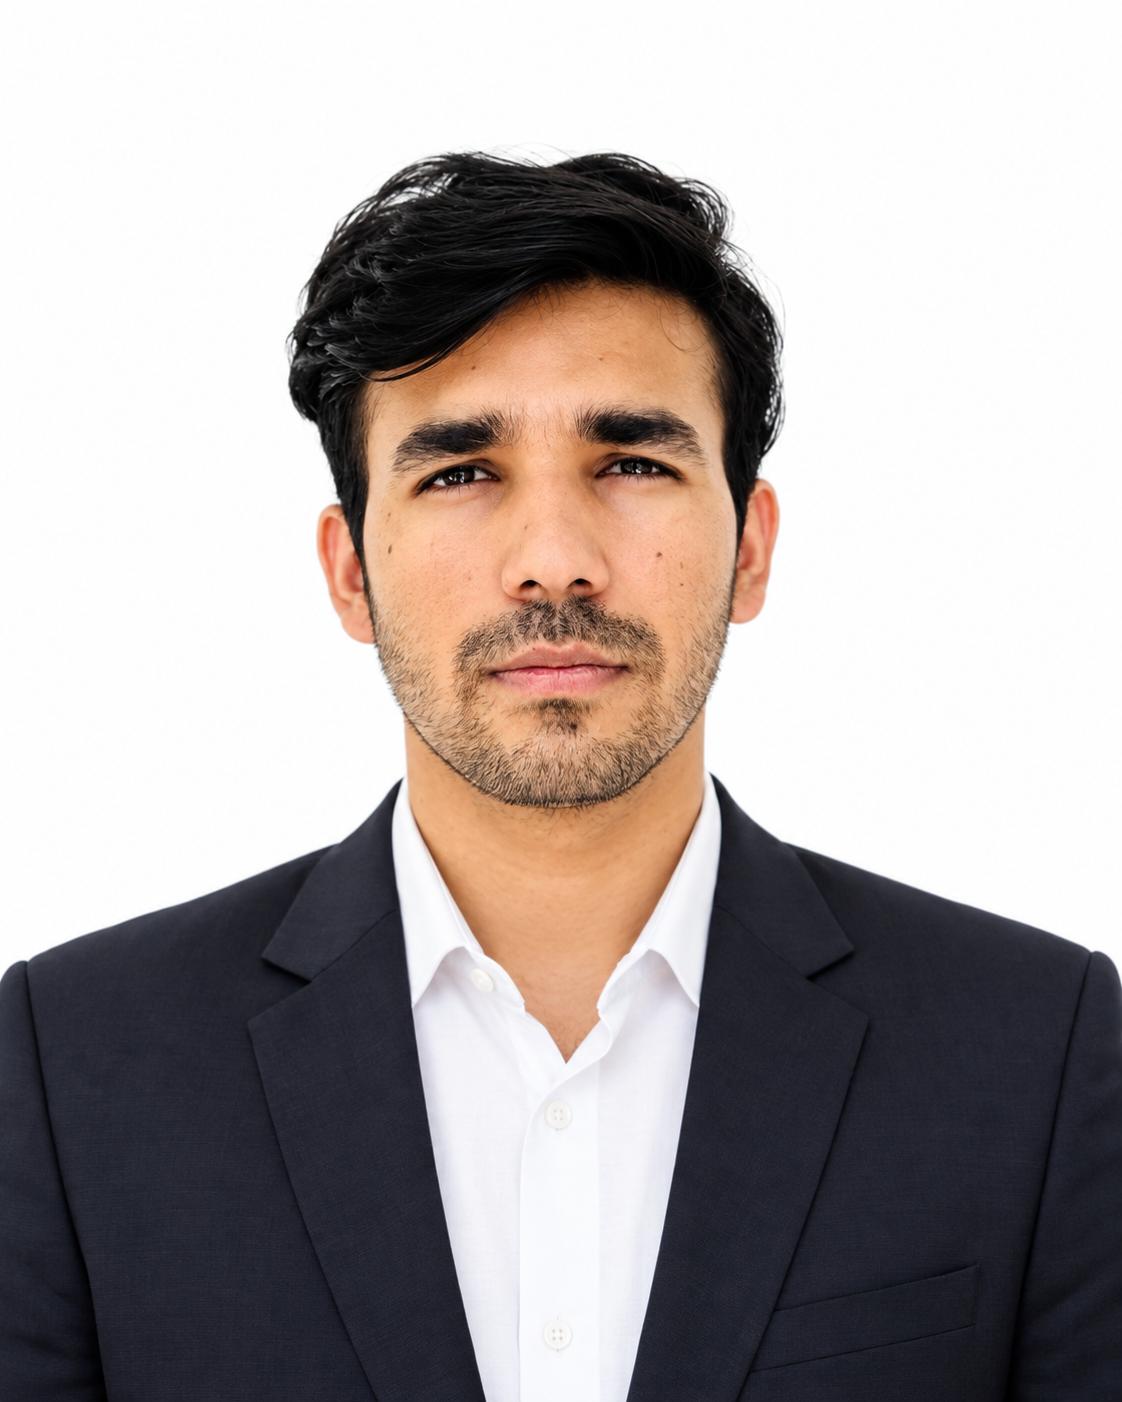
\includegraphics[width=1in,height=1.25in,clip,keepaspectratio]{figures/waseem.png}}]{Waseem Mushtaq}
is pursuing the B.Sc. degree in Computer Science at Albukhary International University, Alor Setar, Kedah, Malaysia, under a fully funded international scholarship. His research interests include machine learning, artificial intelligence, applied data science, and real-world AI systems. His recent work includes applied machine-learning projects and robust evaluation of financial fraud-detection models.
\end{IEEEbiography}

\begin{IEEEbiography}[{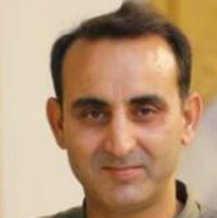
\includegraphics[width=1in,height=1.25in,clip,keepaspectratio]{figures/qaiser.png}}]{Qaiser Abbas}
received the M.S. degree in Computer Science from the National University of Computer and Emerging Sciences, Lahore, Pakistan, in 2010 and completed doctoral studies in Natural Language Processing and Computational Linguistics at the University of Konstanz, Germany, in 2014. He is currently with the Islamic University of Madinah, Madinah, Saudi Arabia. His research covers natural language processing, computational linguistics, machine learning, deep learning, mathematical modelling, and information retrieval. His ORCID is 0000-0003-1870-0884.
\end{IEEEbiography}

\begin{IEEEbiography}[{
\includegraphics[width=1in,height=1.25in,clip,keepaspectratio]{figures/adnan.jpeg}}]{Adnan Nadeem Al Hassan}
(Senior Member, IEEE) received the Ph.D. degree from the University of Surrey, U.K., in 2011. He is a Full Professor and Head of the Department of Computer Science at the Islamic University of Madinah, Madinah, Saudi Arabia.
His work addresses real-world problems using the Internet of Things, advanced imaging, and artificial intelligence in smart cities, healthcare, agriculture, and security. His profile is available at \url{https://adnan-nadeem.com/}.
\end{IEEEbiography}

\begin{IEEEbiography}[{
\includegraphics[width=1in,height=1.25in,clip,keepaspectratio]{figures/abdullah.jpeg}}]{Abdullah Alshanqiti}
received the Ph.D. degree in Computer Science from the University of Leicester, U.K. He is currently with the Faculty of Computer and Information Systems, Islamic University of Madinah, Madinah, Saudi Arabia.
His research interests include artificial intelligence, software engineering, model-driven engineering, responsible AI, federated machine learning, quantum machine learning, knowledge transfer, and image and language understanding.
\end{IEEEbiography}

\begin{IEEEbiography}[{
\includegraphics[width=1in,height=1.25in,clip,keepaspectratio]{figures/sami.jpeg}}]{Sami Albouq}
received the Bachelor's, Master's, and Doctoral degrees in Computer Science in 2009, 2011, and 2018, respectively. He is an Associate Professor with the Faculty of Computer and Information Systems, Islamic University of Madinah, Madinah 42351, Saudi Arabia.
His research interests include system security engineering, complex information technology systems, and quantum key distribution systems. His ORCID is 0009-0007-0955-544X.
\end{IEEEbiography}


\end{document}
